% Generated by build_article.py; edit the modular section files.

% ===== preamble.tex =====
\documentclass[11pt,a4paper]{article}
\usepackage[margin=25mm]{geometry}
\usepackage[T1]{fontenc}
\usepackage{lmodern}
\usepackage{amsmath,amssymb,amsthm,mathtools}
\usepackage{graphicx,booktabs,longtable,array,enumitem,xcolor,microtype,xurl}
\usepackage[colorlinks=true,linkcolor=blue!40!black,citecolor=blue!40!black,urlcolor=blue!50!black]{hyperref}
\usepackage{bookmark}
\emergencystretch=2em
\setcounter{tocdepth}{2}
\numberwithin{equation}{section}
\theoremstyle{plain}
\newtheorem{theorem}{Theorem}[section]
\newtheorem{proposition}[theorem]{Proposition}
\newtheorem{lemma}[theorem]{Lemma}
\newtheorem{corollary}[theorem]{Corollary}
\newtheorem{conjecture}[theorem]{Conjecture}
\theoremstyle{definition}
\newtheorem{definition}[theorem]{Definition}
\theoremstyle{remark}
\newtheorem{remark}[theorem]{Remark}
\newtheorem{example}[theorem]{Example}
\DeclareMathOperator{\Li}{Li}
\DeclareMathOperator{\rank}{rank}
\DeclareMathOperator{\ord}{ord}
\DeclareMathOperator{\lcm}{lcm}
\newcommand{\src}[1]{\nolinkurl{#1}}
\newcommand{\dd}{\,\mathrm d}
\title{Uniform Transitions and Integral Structures\\[4pt]
in Polylogarithmic Analysis\\[10pt]
\large A research continuation of the ProveIt manuscript}
\author{ProveIt Contributors}
\date{10 October 2026}
\hypersetup{pdftitle={Uniform Transitions and Integral Structures in Polylogarithmic Analysis},pdfauthor={ProveIt Contributors},pdfsubject={Research continuation: harmonic saddles, reflected gamma moments, integral distribution lattices and Gaussian identities}}


% ===== frontmatter.tex =====
\begin{document}
\maketitle
\begin{abstract}
We extend three parts of the ProveIt polylogarithms programme and
reconcile an outstanding pair of weight-seven candidates. For
alternating harmonic sums, a rescaled saddle and a global gamma-phase
majorant give a relative expansion at every fixed order, uniform for
all depths and all positive shifts as the outer exponent grows.
We invert the first-pole transition and obtain explicit logarithmic
corrections to its threshold. For reflected log-gamma moments with
both exponents growing, we prove a nontrivial transition factor,
its first two corrections, and exact coefficient identities at
every order. An exact interval certificate also proves global
monotonicity of a reflected log-gamma slope ratio, giving a unique
nondegenerate saddle and a full expansion for every fixed positive
ratio of the two exponents. For weighted distribution relations, an explicit
integral grid basis supports a complete two-prime primitive-cokernel
calculation, including torsion, modular ranks, Smith factors, and
optimal rational reduction denominators. Explicit level-fifteen
Hurwitz-zeta identities follow. Two convergent shuffles prove that
the two recorded $S_6$ candidates are equivalent; the common
evaluation remains conjectural. Full proofs, exact verifiers,
clearly classified numerical diagnostics, source receipts,
editorial corrections, and a further research programme accompany
the article.
\end{abstract}
\medskip
\noindent\textbf{Keywords.} Multiple polylogarithms; alternating harmonic
sums; Laplace asymptotics; gamma moments; universal distributions;
Smith normal form; Hurwitz zeta; exact certificates.
\medskip
\par\noindent\textbf{Baseline.} Immutable repository commit
\texttt{cc34f73596336f2466d9754cb0f3635bd2bedade}, including the six
incoming archives deposited with it. Results are distinguished from
that existing material throughout.
\clearpage
\begingroup
\small
\linespread{0.95}\selectfont
\tableofcontents
\endgroup
\clearpage


% ===== sections/01-introduction.tex =====
\section{Scope, conventions, and principal results}
\label{cont:sec:introduction}

This article continues the research programme in \emph{Polylogarithms
and their Arithmetic Bridges} at the immutable ProveIt commit
\texttt{cc34f73596336f2466d9754cb0f3635bd2bedade}, dated
10 October 2026 \cite{cont:ProveIt}. The baseline includes both the
consolidated manuscript and six newly deposited research archives.
This distinction matters: several conjectures still labelled open in
the consolidated text already have proofs in those incoming archives.
The present contribution does not count those proofs as new work.
An accompanying inventory records the exact source and archive hashes.

The results concern three structures which recur throughout the
programme. Positive Mellin integrals control alternating harmonic sums;
gamma concentration describes a transition in reflected log-gamma
moments; integral distribution relations organize rational-grid special
values. A shorter fourth part reconciles the two recorded weight-seven
Gaussian candidates by an exact shuffle identity. The proofs are analytic
and algebraic, with one explicitly identified computer-assisted inequality
whose finite middle-interval step uses exact integer arithmetic. Other
computations supply reproducible checks and examples, and are identified
explicitly when they provide only numerical evidence.

\subsection{What is already known in the pinned material}

The consolidated manuscript already proves the mixed Gaussian
$S_4$ evaluation, signed first-omitted-term bounds for the harmonic
family, its first-pole transition, an all-orders expansion within that
transition, and a saddle expansion when the exponent-to-depth ratio
stays in a fixed positive compact interval. Its reflected log-gamma
theory includes fixed-reflected-exponent expansions, late coefficients,
and a sharp optimal-truncation remainder. Its distribution theory
includes arbitrary complex weights, conductor coordinates, exceptional
spectral jets, and a primitive-grid determinant up to a constant from
the choice of complex coordinates.

The six incoming archives additionally include proofs of the odd-weight
rank conjecture for the signed depth-two product module, extensions to
other levels, integral Smith calculations for that product module,
independent $S_4$ certificates, complement-collision classifications,
CM evaluations, and further zero-geometry results. These are distinct
from the integral distribution lattice studied here. A small apparent
coefficient relation found numerically at a higher weight is not made
a theorem by being stored in an incoming report. In particular, both
recorded $S_6$ formulas remain conjectural.

\subsection{The contributions proved here}

\begin{enumerate}[leftmargin=*,label=\arabic*.]
\item \textbf{A single harmonic saddle over the whole moving range.}
Theorem~\ref{us:thm:uniform} gives an all-orders \emph{relative}
expansion as $p\to\infty$, uniformly for all integers $h\ge1$ and
all $a>0$. It allows $p/h$ to tend to zero, to remain bounded, or to
grow without bound. The exact saddle incorporates the shift $a$.
A global gamma-phase upper bound makes this uniformity possible.
This resolves the request in the proportional-depth chapter for an
approximation which continues through the growing-ratio transition.

\item \textbf{An inverse transition with explicit corrections.}
Theorem~\ref{us:thm:inverse} determines the unique real outer exponent
at which the normalized harmonic sum reaches a prescribed value
$\theta\in(0,1)$. It gives a finite recursion to every order and
prints the first two correction polynomials. Its error is proved by
asymptotic brackets, without differentiating an unspecified remainder.

\item \textbf{A transition when both reflected moment exponents grow.}
Theorem~\ref{joint:thm:transition} treats
$(n+1)/(m+1)=\log m+O(1)$ with $m\to\infty$. The fixed-$m$
endpoint formula acquires a surviving factor
\[
 \exp\!\left[\left(\frac{\zeta(2)}{2\gamma}-\gamma\right)
       m\exp\!\left(-\frac{n+1}{m+1}\right)\right].
\]
Two corrections and an all-orders coefficient rule are proved.
Corollary~\ref{joint:cor:top-coefficients} gives exact identities for
two extremal coefficient families in every order.

\item \textbf{A unique saddle for every proportional moment.}
Theorem~\ref{gs:thm:monotonicity} proves that
\[
 x\longmapsto
 \frac{-\psi(x)\log\Gamma(1-x)}
      {-\psi(1-x)\log\Gamma(x)}
\]
is strictly increasing on $(0,1)$. The proof combines analytic
endpoint estimates with a small exact rational interval certificate.
Theorem~\ref{gs:thm:proportional} consequently gives the complete
moment expansion for exponent ratios in any compact positive
interval, including a unique nondegenerate saddle. This settles
another part of the simultaneous large-exponent problem.

\item \textbf{Integral coordinates and the complete two-prime
primitive cokernel.} Theorem~\ref{intdist:thm:basis} gives a concrete
grid basis over every commutative coefficient ring. Its finite
resolution is an explicit adaptation of classical universal-distribution
methods. The principal additional calculation is
Theorem~\ref{intdist:thm:two-prime}: a complete presentation of the
primitive-grid cokernel at $q=p\ell$, including torsion at singular
weights. Its Smith factors give the exact denominator required to
express all grid points in primitive coordinates. Explicit level-fifteen
Hurwitz-zeta identities illustrate the result.

\item \textbf{An exact reconciliation of the weight-seven
candidates.} Proposition~\ref{s6audit:prop:coordinate} proves a
coordinate identity among Gaussian doubles and shows that the two
$S_6$ candidates are the same conjecture. The displayed certificate
uses two convergent shuffles. An incomplete larger relation search
is reported as inconclusive.
\end{enumerate}

The phrase ``additional result'' means an extension of the audited
baseline, with the antecedents stated below. It is not a claim of
global priority after an exhaustive literature search. In particular,
the freeness/resolution principle in universal distributions is
classical; its role here is to support explicit integral calculations,
not to rename an existing general theory.

\subsection{Notation and interpretation}

We use $\gamma$ for Euler's constant and
$\beta(s)=\sum_{n\ge0}(-1)^n(2n+1)^{-s}$ for the Dirichlet beta
function when the defining series converges. The multiple-polylogarithm
convention is
\[
 \operatorname{Li}_{s_1,\ldots,s_d}(z_1,\ldots,z_d)
 =\sum_{n_1>\cdots>n_d\ge1}
    \frac{z_1^{n_1}\cdots z_d^{n_d}}
         {n_1^{s_1}\cdots n_d^{s_d}},
\]
continued only where a continuation is expressly indicated. All
Gaussian shuffles used for the coordinate theorem converge ordinarily.
The normalized harmonic quantity $R_{p,h}$ and the normalized moment
$\mathcal R_{n,m}$ are different functions. The symbol $\lambda$ is a
local transition parameter defined separately in each section.

The term \emph{formal distribution module} refers to symbols subject
to specified linear multiplication relations. Its rank is not the
dimension of the span of the corresponding evaluated special values.
Similarly, a Smith factor describes a particular integral inclusion;
it is not an assertion of algebraic or transcendence independence.
These distinctions are essential at exceptional weights and in finite
characteristic.

\subsection{Reading and integration guide}

Sections~\ref{us:sec:uniform}--\ref{us:sec:inverse} extend the harmonic
chapters. Sections~\ref{joint:sec:moments}--\ref{gs:sec:main} belong
after the fixed-$m$ reflected-moment and sharp-remainder material.
Section~\ref{intdist:sec:main} supplements the distribution and
conductor chapters. Section~\ref{s6audit:sec:main} belongs beside the
weight-seven conjecture. Section~\ref{cont:sec:editorial} records
proposed corrections and status changes; the final sections describe
the computational evidence and a prioritized research agenda.
The archive includes both an assembled \TeX{} article and modular
section files, together with exact verifiers, numerical diagnostics,
source receipts, and a small proposed editorial patch.


% ===== sections/02-uniform-harmonic.tex =====
\section{A single harmonic saddle throughout the moving range}
\label{us:sec:uniform}

For an integer $h\ge1$ define
\[
 e_h(n)=[u^h]\prod_{j=1}^n(1+u/j),\qquad
 T_{p,h}(a)=\sum_{n\ge0}\frac{(-1)^ne_h(n)}{(n+a)^p},
 \qquad p,a>0.
\]
The empty product is one, so $e_h(n)=0$ for $n<h$ and
$e_h(h)=1/h!$. In particular $e_1(n)=H_n$. The first nonzero
term of the alternating series motivates the normalization
\begin{equation}\label{us:eq:R}
 R_{p,h}(a)=(-1)^hh!(h+a)^pT_{p,h}(a).
\end{equation}
For $a=1/2$, the Gaussian harmonic family in the manuscript is
$S_{p,h}=2^{-p}T_{p,h}(1/2)$; its usual $S_p$ means $S_{p,1}$.

\subsection{The exact positive integral}

We briefly justify the starting point to keep the asymptotic argument
self-contained. The generating function is
\begin{equation}\label{us:eq:generating}
 \sum_{n\ge0}e_h(n)z^n
 =\frac{(-\log(1-z))^h}{h!(1-z)},\qquad |z|<1.
\end{equation}
It follows by taking the coefficient of $u^h$ in
$\sum_{n\ge0}\prod_{j=1}^n(1+u/j)z^n=(1-z)^{-1-u}$.
Ordinary convergence of $T_{p,h}$ for $p>0$ can also be checked
directly. The recurrence
$e_h(n)-e_h(n-1)=e_{h-1}(n-1)/n$ and
$e_h(n)=O_h((1+\log n)^h)$ show that
$e_h(n)/(n+a)^p\to0$ and its successive differences have an
absolutely summable majorant of order
$n^{-p-1}(1+\log n)^h$. Summation by parts against $(-1)^n$
therefore proves convergence. Absolute convergence holds for $p>1$.

Insert an Abel factor $0<\rho<1$ in the sum and use
$(n+a)^{-p}=\Gamma(p)^{-1}\int_0^\infty y^{p-1}e^{-(n+a)y}\,dy$.
Equation~\eqref{us:eq:generating} and dominated convergence as
$\rho\uparrow1$ give
\begin{equation}\label{us:eq:integral}
 R_{p,h}(a)=\frac{(h+a)^p}{\Gamma(p)}
 \int_0^\infty
  \frac{y^{p-1}e^{-ay}L(y)^h}{1+e^{-y}}\,dy,
 \qquad L(y)=\log(1+e^{-y}).
\end{equation}
The bound $L(y)\le\min(\log2,e^{-y})$ controls both endpoints.
This integral, including its positivity, is already established in
the manuscript \cite[\src{chapters/04-depth.tex},
\src{chapters/04-proportional-depth.tex}]{cont:ProveIt}.

Define
\[
 k_h(t)=\frac1{1+t}\left(\frac{\log(1+t)}t\right)^h,
 \quad k_h(0)=1.
\]
If $Y_p$ has the gamma law with shape $p$ and rate $h+a$, then
\begin{equation}\label{us:eq:gamma}
 R_{p,h}(a)=\mathbb E k_h(e^{-Y_p}).
\end{equation}
The kernel $k_h$ is strictly decreasing on $[0,1]$, with
$k_h(1)=(\log2)^h/2$ and $k_h(0)=1$. Consequently
\begin{equation}\label{us:eq:bounds}
 \frac{(\log2)^h}{2}<R_{p,h}(a)<1.
\end{equation}

\subsection{The moving saddle and the uniform expansion}

Put
\[
 w(y)=-\frac{d}{dy}\log L(y)
     =\frac1{(1+e^y)L(y)},\qquad
 \alpha=p/h,\qquad \epsilon=a/h.
\]
Writing $v=e^{-y}$ gives
\[
 \frac{d}{dv}\log\frac{v}{(1+v)\log(1+v)}
 =\frac{\log(1+v)-v}{v(1+v)\log(1+v)}<0.
\]
Thus $w$ increases strictly from $w_0=1/(2\log2)$ to $1$.
There is exactly one $x>0$ satisfying
\begin{equation}\label{us:eq:saddle}
 x(w(x)+\epsilon)=\alpha,
 \qquad
 \frac{p}{h+a}<x<\frac{p}{hw_0+a}.
\end{equation}
This is the saddle for the full exponent after absorbing the
factor $e^{-ay}$ into it. Keeping $a$ in the exponent is useful when
$a$ itself varies.

At this $x$ set
\begin{align}
 B&=1+\frac{x^2w'(x)}{\alpha},
 &A(z)&=\frac1{z(1+e^{-xz})},\label{us:eq:BA}\\
 \Psi(z)&=\log z+
  \frac{\log L(xz)-\log L(x)-\epsilon x(z-1)}\alpha.
 \label{us:eq:phase}
\end{align}
Then $\Psi(1)=\Psi'(1)=0$ and $\Psi''(1)=-B$.

\begin{theorem}[Uniform expansion with no ratio restriction]
\label{us:thm:uniform}
For each fixed integer $J\ge0$, as $p\to\infty$, uniformly over
all integers $h\ge1$ and all real $a>0$,
\begin{equation}\label{us:eq:uniform}
 R_{p,h}(a)=\mathcal S_{p,h}(a)
 \left\{\sum_{j=0}^J\frac{E_j(x,\epsilon)}{p^j}
       +O_J(p^{-J-1})\right\},
\end{equation}
where $E_0=1$ and
\begin{equation}\label{us:eq:prefactor}
 \mathcal S_{p,h}(a)=
 \frac{((h+a)x)^p e^{-ax}L(x)^h}
      {\Gamma(p)(1+e^{-x})}
 \sqrt{\frac{2\pi}{pB}}.
\end{equation}
Every coefficient $E_j$ is bounded on the entire parameter range.
In particular, with all derivatives evaluated at $z=1$,
\begin{equation}\label{us:eq:E1}
 E_1=\frac{A''}{2BA}
      +\frac{\Psi'''A'}{2B^2A}
      +\frac{\Psi''''}{8B^2}
      +\frac{5(\Psi''')^2}{24B^3}.
\end{equation}
The constants in the relative remainder depend on $J$ alone.
\end{theorem}

\begin{proof}
Substitute $y=xz$ in \eqref{us:eq:integral}. After removing its
value at the saddle, the remaining integral is
\begin{equation}\label{us:eq:reduced-integral}
 \int_0^\infty e^{p\Psi(z)}A(z)\,dz.
\end{equation}
We verify the uniform conditions for Laplace expansion directly.
The local expansion itself is the usual one
\cite[\S2.3(iii)]{cont:DLMFLaplace}; the global parameter control is
the point requiring proof here.

First, the concavity of $\log L$, equivalent to $w'>0$, gives its
tangent bound at $x$. Combining this bound with the saddle equation
yields the parameter-free majorant
\begin{equation}\label{us:eq:majorant}
 \boxed{\displaystyle \Psi(z)\le\log z-z+1\quad(z>0).}
\end{equation}
Also $A(z)\le z^{-1}$. For each fixed $0<d<1$, the contribution
of $|z-1|\ge d$ to \eqref{us:eq:reduced-integral} is bounded by
the corresponding tail of
$e^p\int_0^\infty z^{p-1}e^{-pz}\,dz$.
The gamma Chernoff bound, followed by Stirling's formula, bounds
that tail by $C_dp^{-1/2}e^{-c_dp}$ for positive constants
independent of $h$ and $a$.

Second, the saddle curvature is bounded above and below uniformly.
For $r_x=(1+e^x)^{-1}$, logarithmic differentiation gives
$w'=w(w-1+r_x)$, hence $0<w'\le r_x\le e^{-x}$.
Therefore
\begin{equation}\label{us:eq:curvature-bound}
 1\le B=1+\frac{xw'(x)}{w(x)+\epsilon}
 \le1+\frac{2\log2}{e},
 \qquad \frac12\le A(1)\le1.
\end{equation}
For $z$ in any fixed closed neighborhood of $1$ contained in
$(0,\infty)$, every fixed derivative of $A$ is uniformly bounded.
For $k\ge2$, the nonlogarithmic part of $\Psi^{(k)}(z)$ has
absolute value
\begin{equation}\label{us:eq:derivative-control}
 \frac{x^k|w^{(k-1)}(xz)|}{\alpha}
 =\frac{x^{k-1}|w^{(k-1)}(xz)|}{w(x)+\epsilon}.
\end{equation}
Near $x=0$, the analyticity of $w$ and $w\ge w_0$ bound this
expression. As $x\to\infty$, use
$w^{(j)}(u)=O_j(e^{-u})$ for $j\ge1$ and the boundedness of
$x^je^{-cx}$ for fixed $j$ and $c>0$. These observations also
prove the required bounds for the logistic amplitude. The linear
$\epsilon$ term has disappeared from all derivatives of order
at least two; increasing $\epsilon$ only increases the denominator
in \eqref{us:eq:derivative-control}. This explains why no upper
bound on $a$ is needed.

Finally,
$\Psi''(z)=-z^{-2}-x^2w'(xz)/\alpha\le-z^{-2}$.
On the fixed saddle neighborhood this supplies a common Gaussian
bound after $z=1+u/\sqrt p$. To any fixed order one may Taylor
expand the phase and amplitude there, retaining enough derivatives
to bound the remainder by $p^{-J-1}$ times a fixed integrable
polynomial times a Gaussian. One explicit justification is to first
restrict to $|u|\le p^\nu$, with a sufficiently small positive
$\nu$ depending on the desired order, expand to a higher finite
Taylor order, and use the common Gaussian bound on its complement.
All derivative bounds and all choices are independent of the
parameters. Extending each retained Gaussian monomial to the real
line incurs an exponentially small error. Odd monomials integrate
to zero. The even moments give
\[
 \int_0^\infty e^{p\Psi(z)}A(z)\,dz
 =A(1)\sqrt{\frac{2\pi}{pB}}
   \left\{\sum_{j=0}^J E_jp^{-j}+O_J(p^{-J-1})\right\}.
\]
Restoring the exact prefactor proves \eqref{us:eq:uniform}.
Taking the four possible even Gaussian contributions at order
$p^{-1}$ gives \eqref{us:eq:E1}.
\end{proof}

There is a finite prescription for every coefficient. Let
$\mathbb E_B$ denote expectation under a centered normal law of
variance $1/B$, and let $\tau$ be formal. Then
\begin{equation}\label{us:eq:coefficient-recipe}
 E_j=\frac1{A(1)}[\tau^{2j}]
 \mathbb E_B\!\left[
 A(1+\tau u)
 \exp\!\left(\sum_{k\ge3}
      \frac{\Psi^{(k)}(1)}{k!}u^k\tau^{k-2}\right)\right].
\end{equation}
Coefficient extraction precedes Gaussian integration. Only finitely
many derivatives and moments enter, so this is an exact algorithm
for any prescribed order, not an assertion that the complete
asymptotic series converges.

\subsection{Evaluation, overlaps, and limitations}

For the first correction, useful formulas are
\begin{align}
 \frac{A'(1)}{A(1)}&=-1+xr_x,&
 \frac{A''(1)}{A(1)}&=2-2xr_x+x^2(2r_x^2-r_x),\label{us:eq:amplitude-derivatives}\\
 \Psi'''(1)&=2-\frac{x^3w''(x)}\alpha,&
 \Psi''''(1)&=-6-\frac{x^4w'''(x)}\alpha.
 \label{us:eq:phase-derivatives}
\end{align}
As $x\to0$ or $x\to\infty$, $E_1\to1/12$ uniformly in
$\epsilon\ge0$. In the genuine first-pole limit, for example fixed
$h,a$ and $p\to\infty$, this correction cancels the first reciprocal
Stirling correction in the prefactor, consistently with $R\to1$.
The condition $x\to\infty$ alone is insufficient for that conclusion
when $h$ grows. For instance $p/h=\tfrac12\log h$, with fixed $a$,
still lies below the first-pole threshold and gives $R\to0$.

The theorem includes several formerly separate ranges:
$h=p^3$ gives $p/h\to0$; $h\asymp p$ gives a proportional
ratio; $p\asymp h\log h$ gives the first-pole transition; and fixed
$h$ gives an unbounded ratio. It also permits shifts such as
$a=p^2$. It does not cover a bounded outer exponent $p$. That
regime retains the separate endpoint expansion in the manuscript.
Nor does an $O_J$ theorem itself supply a certified numerical
constant at a specified small $p$.

For numerical work, compute $\log\mathcal S$ and standardize around
the saddle, rather than directly forming quantities which may be
exponentially small. The accompanying program uses
$u=\sqrt{pB}(z-1)$ in the exact integral. Table~\ref{us:tab:saddle}
reports selected checks; its last column is the absolute discrepancy
in the normalized bracket, $|R/\mathcal S-1-E_1/p|$.

\begin{table}[htbp]
\centering
\caption{Diagnostics for the uniformly scaled saddle formula.
Values come from 50-digit quadrature and are not interval bounds.}
\label{us:tab:saddle}
\begin{tabular}{@{}rrrrr@{}}
\toprule
$p$ & $h$ & $a$ & $|R/\mathcal S-1|$ & $|R/\mathcal S-1-E_1/p|$\\
\midrule
40 & $64000$ & $1/2$ & $2.08546\cdot10^{-3}$ & $2.12816\cdot10^{-6}$\\
160 & $4096000$ & $1/2$ & $5.20968\cdot10^{-4}$ & $1.34979\cdot10^{-7}$\\
40 & 40 & $1/2$ & $4.91662\cdot10^{-4}$ & $1.05027\cdot10^{-5}$\\
160 & 160 & $1/2$ & $1.15818\cdot10^{-4}$ & $6.80536\cdot10^{-7}$\\
160 & 1 & $1/2$ & $5.20968\cdot10^{-4}$ & $1.34979\cdot10^{-7}$\\
40 & 40 & 1600 & $2.08539\cdot10^{-3}$ & $2.12726\cdot10^{-6}$\\
\bottomrule
\end{tabular}
\end{table}

At $(p,h,a)=(160,4096000,1/2)$ the logarithm of the leading
prefactor is about $-1.501185\cdot10^6$. Relative asymptotics remain
informative even there. The finite test set is a check on signs,
normalizations, and the predicted order of error; the parameter-wide
statement follows from the proof, not from these samples.


% ===== sections/03-inverse-harmonic.tex =====
\section{Reversing the first-pole transition}
\label{us:sec:inverse}

The forward transition answers how close an alternating harmonic sum
is to its first term. The inverse question is equally natural: how
large must the real outer exponent be to attain a specified normalized
fraction? The monotonicity needed to pose this question is exact.

\begin{lemma}[Strict order in the outer exponent]
\label{us:lem:monotone}
For fixed $h\ge1$ and $a>0$, the function $p\mapsto R_{p,h}(a)$
is continuous and strictly increasing on $(0,\infty)$, with endpoint
limits $(\log2)^h/2$ and $1$.
\end{lemma}
\begin{proof}
For $d>0$, independent gamma variables with common rate $h+a$
can be coupled by $Y_{p+d}=Y_p+Y_d$. Since
$y\mapsto k_h(e^{-y})$ is strictly increasing and $Y_d>0$
almost surely, \eqref{us:eq:gamma} proves strict increase.
As $p\downarrow0$, $Y_p\to0$ in probability, for instance by its
mean. As $p\to\infty$, $Y_p\to\infty$ in probability by its
mean and variance. The bounded continuous kernel gives the two
limits. The same gamma representation, or dominated convergence
in \eqref{us:eq:integral} on compact $p$-intervals, gives continuity.
\end{proof}

For $0<\theta<1$ put
\begin{equation}\label{us:eq:inverse-parameters}
 \lambda=-\log\theta,
 \qquad L_0=\log h-\log(2\lambda).
\end{equation}
For all sufficiently large $h$, Lemma~\ref{us:lem:monotone}
therefore gives a unique $p_\theta(h,a)>0$ satisfying
$R_{p_\theta,h}(a)=\theta$.

\begin{theorem}[All-orders inverse transition]
\label{us:thm:inverse}
Fix compact intervals of $a$ in $(0,\infty)$ and of $\theta$
in $(0,1)$. For every fixed integer $J\ge0$,
\begin{equation}\label{us:eq:inverse-all}
 p_\theta(h,a)=hL_0+
   \sum_{j=0}^J\frac{Q_j(L_0;\lambda,a)}{h^j}
   +O_J\!\left(\frac{L_0^{J+2}}{h^{J+1}}\right),
 \qquad h\to\infty,
\end{equation}
uniformly on those intervals. Here $Q_j\in\mathbb Q[L_0,\lambda,a]$
has degree at most $j+1$ in $L_0$. The first two polynomials are
\begin{align}
 Q_0(L;\lambda,a)
  & =\left(a+\frac12-\frac\lambda2\right)L
       +2-\frac{5\lambda}{6},\label{us:eq:Q0}\\
 Q_1(L;\lambda,a)
  & =\left(\frac{\lambda^2}{8}-\frac\lambda4\right)L^2
    +\left(\frac{\lambda^2}{3}-\frac\lambda3-\frac1{12}\right)L
       \notag\\
  &\hspace{1.5em}-\frac{5a\lambda}{6}+2a
       +\frac{3\lambda^2}{8}-\frac\lambda{12}-1.
       \label{us:eq:Q1}
\end{align}
\end{theorem}

\subsection{The forward coefficients used in the inversion}

We state the input with its provenance, since it is already proved in
the baseline. Write $L=p/h$ and $v=he^{-L}/2$. In the compact
transition window $L=\log h+O(1)$, the all-orders compiler of
\cite[\src{chapters/04-depth.tex}, Theorem
\texttt{harmonic:thm:allorders}]{cont:ProveIt} gives
\begin{equation}\label{us:eq:forward}
 R_{p,h}(a)=e^{-v}
    \sum_{j=0}^N\frac{\Theta_j(L,v;a)}{h^j}
       +O_N\!\left(\frac{L^{N+1}}{h^{N+1}}\right).
\end{equation}
Each $\Theta_j$ has degree at most $j$ in $L$, and
\begin{equation}\label{us:eq:Theta1}
 \Theta_0=1,
 \qquad
 \Theta_1=\left(\frac{v^2}{2}-(a+\tfrac12)v\right)L
              +\frac56v^2-2v.
\end{equation}
A finite way to regenerate these polynomials is as follows. Set
\[
 \mathcal D P(v)=vP(v)-vP'(v),\qquad
 d_j(t;a)=\frac{(-1)^j}{j+1}
                \{a^{j+1}-(a-t)^{j+1}\}.
\]
Define $\mathcal U_j$ by the formal kernel expansion
\[
 k_h(2v/h)=e^{-v}\sum_{j\ge0}\mathcal U_j(v)h^{-j}.
\]
Then, as a formal power series in $z$,
\begin{equation}\label{us:eq:forward-recipe}
 \sum_{j\ge0}\Theta_j(L,v;a)z^j
 =\exp\!\left(L\sum_{k\ge1}z^k d_k(\mathcal D;a)\right)
       \sum_{k\ge0}\mathcal U_k(v)z^k.
\end{equation}
All operations truncate after finitely many terms at a requested
order. For example
$\mathcal U_1=5v^2/6-2v$ and
$\mathcal U_2=25v^4/72-8v^3/3+4v^2$.
The exact gamma cumulant identity behind the compiler is
\[
 \log\mathbb E e^{t(Y_p-L)}
 =-Lt+hL\{\log(1+a/h)-\log(1+(a-t)/h)\}.
\]
Thus the forward coefficient rule is algebraic, and its uniform
error comes from bounded kernel derivatives and centered gamma moments.

\subsection{Formal inversion and a rigorous error bracket}

\begin{proof}[Proof of Theorem~\ref{us:thm:inverse}]
Set $z=1/h$ and write $p/h=L_0+\delta$, so $v=\lambda e^{-\delta}$.
The formal equation for the inverse is
\begin{equation}\label{us:eq:implicit}
 0=\lambda-\lambda e^{-\delta}
   +\log\!\left(
        \sum_{j\ge0}z^j
          \Theta_j(L_0+\delta,\lambda e^{-\delta};a)\right).
\end{equation}
It has a unique solution
$\delta=\sum_{j\ge0}z^{j+1}Q_j(L_0;\lambda,a)$ because its
coefficient of $\delta$ at $z=0,\delta=0$ is $\lambda\ne0$.
The recursion is effective: substitute known coefficients and divide
the next residual coefficient by $-\lambda$.

There are no hidden denominators in $\lambda$. For $j>0$ every
$\Theta_j(L,v;a)$ is divisible by $v$: this follows directly
from \eqref{us:eq:forward-recipe}, since $\mathcal D$ preserves
the ideal $(v)$, $d_k(0;a)=0$, and $\mathcal U_j(0)=0$ for $j>0$.
The logarithm in
\eqref{us:eq:implicit} is therefore coefficientwise divisible by
$\lambda$. After division the derivative with respect to $\delta$
is one. Induction gives $Q_j\in\mathbb Q[L_0,\lambda,a]$.
The bound on the degree in $L_0$ follows by the same induction:
a term of order $z^r$ has degree at most $r$ in $L_0$, including
products and the substitutions in \eqref{us:eq:implicit}.

At order $z$, the equation is
$\lambda Q_0+\Theta_1(L_0,\lambda;a)=0$, proving
\eqref{us:eq:Q0}. At order $z^2$ it gives
\[
 Q_1=\frac{Q_0^2}{2}
  -\frac{
     Q_0(\partial_L-\lambda\partial_\lambda)\Theta_1
       +\Theta_2-\Theta_1^2/2}{\lambda},
\]
evaluated at $(L_0,\lambda;a)$. Expanding the forward compiler
through order two gives \eqref{us:eq:Q1}. The accompanying exact
program checks these cancellations both in the logarithmic equation
and in the original normalized expression. A second program derives
the same answer directly from gamma cumulants after shifting $p$.

For the analytic error, let
$p_* = hL_0+\sum_{j=0}^Jh^{-j}Q_j$ and use
\eqref{us:eq:forward} through order $J+1$. The formal
cancellations prove
\[
 R_{p_*,h}(a)-\theta
 =O\!\left(h^{-J-2}L_0^{J+2}\right)
\]
uniformly on the stated compact sets. Apply the same finite expansion
at $p_*\pm K h^{-J-1}L_0^{J+2}$, with $K>0$ fixed.
The leading term changes by
\[
 \pm\theta\lambda K h^{-J-2}L_0^{J+2}(1+o(1)),
\]
and the change of the finitely many correction terms is of smaller
relative order. Since $\theta\lambda$ is bounded away from zero
on a compact subinterval of $(0,1)$, taking $K$ sufficiently large
places the two expanded values on opposite sides of $\theta$.
Both exponents remain in the same compact transition window.
Lemma~\ref{us:lem:monotone} then brackets the unique inverse
between them, proving \eqref{us:eq:inverse-all}. No derivative of
the remainder in \eqref{us:eq:forward} has been assumed.
\end{proof}

\subsection{A quantitative example}

For $\theta=1/2$ and $a=1/2$, numerical inversion of the exact
positive integral gives the values in Table~\ref{us:tab:inverse}.
The final three columns report absolute exponent errors, successively
using $hL_0$, $hL_0+Q_0$, and $hL_0+Q_0+Q_1/h$.
These are high-precision diagnostics of the defining integral,
not interval-certified root enclosures.

\begin{table}[htbp]
\centering
\caption{The inverse harmonic transition at $\theta=a=1/2$.}
\label{us:tab:inverse}
\begin{tabular}{@{}rrrrr@{}}
\toprule
$h$ & numerical $p_{1/2}$ & leading error & with $Q_0$ & with $Q_1/h$\\
\midrule
50 & $182.994297936847$ & $3.72486$ & $4.03044\cdot10^{-2}$ & $3.19479\cdot10^{-3}$\\
200 & $998.989394784027$ & $4.65277$ & $1.82329\cdot10^{-2}$ & $4.26953\cdot10^{-4}$\\
800 & $5091.951714446499$ & $5.56974$ & $7.10744\cdot10^{-3}$ & $4.78128\cdot10^{-5}$\\
\bottomrule
\end{tabular}
\end{table}

The increasing error of the leading approximation is expected:
$Q_0$ contains a multiple of $\log h$. The decreasing errors after
correction illustrate why solving only the leading transition profile
can be inadequate even when the forward normalized sum is well
approximated.


% ===== sections/04-joint-moments.tex =====
% Contribution to the polylogarithms continuation.
% Baseline: cc34f73596336f2466d9754cb0f3635bd2bedade.
% Parent document supplies amsmath, amssymb, amsthm, theorem environments.
\section{A uniform transition for two large reflected log-gamma exponents}
\label{joint:sec:moments}

Write
\[
 f(x)=\log\Gamma(x),\qquad
 M_{n,m}=\int_0^1 f(x)^n f(1-x)^m\,dx,
 \qquad n,m\in\mathbb Z_{\geq0}.
\]
The mixed integrals themselves are classical: they occur as
$T_{n+m,n}$ in Amdeberhan et al.\ \cite[Section~5]{gaussian:ACEMKM}.
The pinned manuscript proves a fixed-$m$ expansion, its late coefficients,
and a sharp remainder at optimal truncation. It explicitly leaves the
regime in which both exponents increase as a separate question.
Here we resolve a transition inside that joint regime.

For fixed $m$, the first endpoint term is
\[
 M_{n,m}\sim\frac{\gamma^m n!}{(m+1)^{n+1}}.
\]
When $m$ increases, its first neglected local perturbation has size
$m\exp[-n/(m+1)]$. Thus it can survive in the limit even though the
relevant endpoint $x$ tends to zero. The transition occurs around
$n/m=\log m$. The theorem below gives its complete expansion, with
explicit first and second corrections. In particular, it does not
substitute a growing $m$ into a fixed-$m$ error estimate.

\subsection{The transition theorem and its first two corrections}

Define the exact constants
\begin{align}
 c&=\frac{\zeta(2)}{2\gamma},&
 d&=\frac{\zeta(3)}{3\gamma}-\frac{c^2}{2},&
 e&=\frac{\zeta(4)}{4\gamma}
       -\frac{c\zeta(3)}{3\gamma}+\frac{c^3}{3},\label{joint:eq:constants1}\\
 \delta&=c-\gamma,&
 \varepsilon&=\gamma^2+d,&
 \eta&=e+\frac{\gamma^3}{2}-\frac{\gamma^2\delta}{2}
          +\frac{\gamma\delta^2}{2}-5\gamma\varepsilon.
 \label{joint:eq:constants2}
\end{align}
In particular,
\[
 \delta=0.84767122475766887678\ldots,
 \qquad
 \varepsilon=0.01219631601207367653\ldots.
\]
The definitions, rather than these diagnostic decimals, specify the
constants in all statements. Notice that $\delta>0$; for example,
$\gamma<0.6$ and $\zeta(2)>1.6$ already suffice.

\begin{theorem}[Uniform joint-exponent transition]\label{joint:thm:transition}
Let
\[
 r=m+1,\qquad t=\frac{n+1}{m+1},\qquad
 \lambda=me^{-t},\qquad
 \mathcal R_{n,m}=\frac{(m+1)^{n+1}M_{n,m}}{\gamma^m n!}.
\]
Fix $0<a<b<\infty$. As $m\to\infty$, uniformly over positive
integers $n$ for which $a\leq\lambda\leq b$,
\begin{equation}\label{joint:eq:two-corrections}
 \mathcal R_{n,m}
 =e^{\delta\lambda}
 \left\{1+\frac{P_1(t,\lambda)}m
          +\frac{P_2(t,\lambda)}{m^2}
          +O_{a,b}\left(\frac{t^3}{m^3}\right)\right\},
\end{equation}
where
\begin{equation}\label{joint:eq:P1}
 P_1(t,\lambda)=\frac{t}{2}\delta\lambda(1+\delta\lambda)
                      -2\gamma\lambda+\varepsilon\lambda^2,
\end{equation}
and
\begin{align}
 P_2(t,\lambda)={}&
 \lambda\left\{\frac{\delta t^2}{8}
                    -\left(\gamma+\frac{5\delta}{6}\right)t\right\}
 \notag\\
 &+\lambda^2\left\{\frac{7\delta^2t^2}{8}
        +\left(-3\gamma\delta-\frac{3\delta^2}{2}
                        +2\varepsilon\right)t
        +\frac{15\gamma^2}{2}+3\gamma\delta\right\}\notag\\
 &+\lambda^3\left\{\frac{3\delta^3t^2}{4}
        +\left(-\gamma\delta^2-\frac{\delta^3}{3}
                           +\frac{5\delta\varepsilon}{2}\right)t
        +\eta\right\}\notag\\
 &+\lambda^4\left\{\frac{\delta^4t^2}{8}
                    +\frac{\delta^2\varepsilon t}{2}
                    +\frac{\varepsilon^2}{2}\right\}.
 \label{joint:eq:P2}
\end{align}
More generally, for every fixed integer $J\geq0$, there are explicitly
computable polynomials $P_0=1,P_1,\ldots,P_J$ such that
\begin{equation}\label{joint:eq:all-orders}
 \mathcal R_{n,m}=e^{\delta\lambda}
 \left\{\sum_{\ell=0}^J\frac{P_\ell(t,\lambda)}{m^\ell}
       +O_{a,b,J}\left(\frac{t^{J+1}}{m^{J+1}}\right)\right\}.
\end{equation}
They have degree at most $\ell$ in $t$ and at most $2\ell$ in
$\lambda$, and
\[
 P_\ell\in
 \mathbb Q[\gamma,\gamma^{-1},\zeta(2),\ldots,\zeta(\ell+2)]
 [t,\lambda].
\]
The finite coefficient prescription in
\eqref{joint:eq:polynomial-prescription} below determines every
$P_\ell$.
\end{theorem}

Here $t=\log m-\log\lambda=\log m+O_{a,b}(1)$, so the displayed
remainders are successive powers of $(\log m)/m$.

\begin{corollary}[The surviving correction to the endpoint formula]
\label{joint:cor:limit}
If $m\to\infty$ and
\[
 \frac{n+1}{m+1}-\log m\longrightarrow s\in\mathbb R,
\]
then
\begin{equation}\label{joint:eq:limit}
 \frac{(m+1)^{n+1}M_{n,m}}{\gamma^m n!}
 \longrightarrow
 \exp\left[\left(\frac{\zeta(2)}{2\gamma}-\gamma\right)e^{-s}\right].
\end{equation}
In particular the fixed-$m$ leading term does not have uniform relative
error $o(1)$ on this window. At $s=0$ its missing factor tends to
$e^\delta=2.3342\ldots$.
\end{corollary}
\begin{proof}
Use $\lambda\to e^{-s}$ in \eqref{joint:eq:all-orders} with $J=0$.
The corrections tend to zero because $t/m\to0$.
\end{proof}

\subsection{Exact gamma averaging and localization at the correct endpoint}

Put
\[
 g(x)=\log\Gamma(1+x),\qquad
 B(x)=\log\Gamma(1-x),\qquad
 C(x)=\frac{B(x)}{\gamma x},\quad C(0)=1.
\]
The classical convergent log-gamma expansion
\cite[\S5.7]{joint:DLMF} gives
\begin{align}
 g(x)&=-\gamma x+\frac{\zeta(2)}2x^2
                         -\frac{\zeta(3)}3x^3+O(x^4),\notag\\
 \log C(x)&=cx+dx^2+ex^3+O(x^4).
 \label{joint:eq:local-series}
\end{align}
All these germs are holomorphic in a fixed disk about zero.
For $0<x<1$, log-convexity of $\Gamma$ between $1$ and $2$ implies
\begin{equation}\label{joint:eq:elementary-envelopes}
 0<f(x)\leq-\log x,\qquad
 0<B(x)\leq-\log(1-x).
\end{equation}
After $x=e^{-y}$, the normalized integral is the exact expectation
\begin{equation}\label{joint:eq:expectation}
 \mathcal R_{n,m}=\mathbb E e^{S(Y)},\qquad
 S(y)=n\log\left(1+\frac{g(e^{-y})}{y}\right)
                         +m\log C(e^{-y}),
\end{equation}
where $Y$ has a gamma distribution with shape $q=n+1=rt$ and rate
$r=m+1$. Thus
\[
 \mathbb EY=t,\qquad
 \operatorname{Var}Y=\frac tr.
\]
The powers and logarithms in \eqref{joint:eq:expectation} are real,
since the original factors are positive.

\begin{lemma}[Uniform localization]\label{joint:lem:localization}
Under the compact-$\lambda$ hypotheses of
Theorem~\ref{joint:thm:transition}, there is $\kappa>0$ such that
\begin{equation}\label{joint:eq:localization}
 \mathbb E\left[e^{S(Y)}\mathbf1_{|Y-t|>1}\right]
       =O_{a,b}\left(e^{-\kappa m/t}\right).
\end{equation}
The same estimate holds with $e^{S(Y)}$ replaced by any fixed power
of $|Y-t|$. In particular, the endpoint $x\to1$, corresponding to
$y\to0$, is negligible on the normalization used in the theorem.
\end{lemma}
\begin{proof}
The first summand of $S(y)$ is nonpositive by
\eqref{joint:eq:elementary-envelopes}. Analyticity of $C$ and $C(0)=1$
give a constant $K$ such that
\[
 e^{S(y)}\leq\exp(Kme^{-y})\qquad(y\geq1).
\]
For $y\geq t+1$ this weight is uniformly bounded, and the gamma
Chernoff bound gives a tail $O(e^{-\kappa m/t})$.
For example the gamma rate function is $I(u)=u-1-\log u$, and
$rt I(1+1/t)\geq r/(3t)$ for all sufficiently large $t$.

For the lower tail, let $p(y)$ denote the gamma density and put
$v=t-y$. When $1\leq y\leq t-1$, we have
\[
 \frac{p(t-v)}{p(t)}
  =\exp\{(rt-1)\log(1-v/t)+rv\}
  \leq t\exp\left(-\frac{rv^2}{2t}\right).
\]
Here $1\leq v\leq t-1$, and $me^{-(t-v)}=\lambda e^v$.
The maximum of $e^v/v^2$ on this interval is at one of its endpoints;
consequently
\[
 K\lambda e^v\leq\frac{rv^2}{4t}
 \qquad(1\leq v\leq t-1)
\]
for all sufficiently large $m$, uniformly in $a\leq\lambda\leq b$.
Indeed the two required bounds reduce to $O(1)\leq r/(4t)$ and
$O(m/t^2)\leq r/(4t)$. It follows that the weighted lower-tail
integral over $[1,t-1]$ is at most
\[
 p(t)t^2e^{-r/(4t)}.
\]
Stirling's inequalities give $p(t)=O(\sqrt{r/t})$; the polynomial
factor is absorbed by slightly reducing $\kappa$.

It remains to bound $0<y<1$. Since $1-e^{-y}\geq y/e$ there,
\[
 B(e^{-y})\leq1-\log y,
 \qquad (1-\log y)^m\leq y^{-m}.
\]
Using $f(e^{-y})\leq y$ in the original normalized integral bounds
this part by
\begin{equation}\label{joint:eq:opposite-endpoint}
 \frac{r^{n+1}}{\gamma^m n!}
 \int_0^1 y^n(1-\log y)^m\,dy
 \leq\frac{r^{n+1}}{\gamma^m n!(n-m+1)}.
\end{equation}
Since $n+1=rt$ and $t=\log m+O(1)$, the logarithm of this bound is
\[
 rt(1-\log t)+O(m+\log n),
\]
which is smaller than $-\kappa m/t$ for large $m$.
This also shows directly why the other endpoint cannot compete.
The unweighted gamma estimates, with polynomial factors, follow by
the same density estimates or by Chernoff's inequality with a
slightly smaller exponent.
\end{proof}

\subsection{Derivation of the first two corrections}

Write $U=Y-t$. On $|U|\leq1$, set $x=(\lambda/m)e^{-U}$ and use
\eqref{joint:eq:local-series}. Uniformly there, together with every
fixed number of $U$-derivatives,
\begin{equation}\label{joint:eq:S-expansion}
 S(t+U)=S_0(U)+\frac{S_1(U)}m+\frac{S_2(U)}{m^2}+O(m^{-3}),
\end{equation}
where
\begin{align}
 S_0(U)&=\lambda e^{-U}
       \left(c-\frac{\gamma t}{t+U}\right),\notag\\
 S_1(U)&=-\frac{\gamma\lambda e^{-U}(t-1)}{t+U}
  +\lambda^2e^{-2U}
       \left(d+\frac{\gamma ct}{t+U}
                   -\frac{\gamma^2t}{2(t+U)^2}\right),\notag\\
 S_2(U)&=\lambda^2e^{-2U}(t-1)
       \left(\frac{\gamma c}{t+U}
                    -\frac{\gamma^2}{2(t+U)^2}\right)\notag\\
 &\quad+\lambda^3e^{-3U}
       \left(e-\frac{\gamma t(d+c^2/2)}{t+U}
          +\frac{\gamma^2ct}{(t+U)^2}
          -\frac{\gamma^3t}{3(t+U)^3}\right).
 \label{joint:eq:S012}
\end{align}
The remainders are uniform because $t/(t+U)$ is bounded,
$x=O(m^{-1})$, and $n=O(mt)$. The displayed amplitudes and all their
fixed-order derivatives are uniformly bounded.

The central gamma moments needed for the first correction are
\[
 \mathbb EU=0,\qquad
 \mathbb EU^2=\frac tr,\qquad
 \mathbb EU^3=\frac{2t}{r^2},\qquad
 \mathbb EU^4=\frac{3t^2}{r^2}+\frac{6t}{r^3}.
\]
In particular, for a smooth amplitude $H$ whose first four derivatives
are uniformly bounded on $[-1,1]$, Taylor expansion through the cubic
term, followed by the localization lemma, gives
\[
 \mathbb EH(U)=H(0)+\frac{t}{2m}H''(0)
                        +O(t^2/m^2).
\]
This notation means that $H$ is averaged on the localized interval;
any uniformly bounded extension outside is immaterial up to the
exponentially small error already bounded. The signed third moment is used: an absolute
third-moment estimate would only give an error of order
$(t/m)^{3/2}$.

Since $S_0(0)=\delta\lambda$, the first normalized correction equals
\[
 S_1(0)+\frac t2\bigl(S_0''(0)+S_0'(0)^2\bigr).
\]
The derivatives are
\[
 S_0'(0)=\lambda\left(-\delta+\frac\gamma t\right),\qquad
 S_0''(0)=\lambda\left(\delta-\frac{2\gamma}t
                                   -\frac{2\gamma}{t^2}\right).
\]
Substitution gives \eqref{joint:eq:P1}. The terms involving $1/t$
cancel exactly; this is an algebraic cancellation, not an additional
large-$t$ approximation.

For an independently reproducible second-order calculation, define
\[
 a_j=S_0^{(j)}(0)\quad(1\leq j\leq4),\qquad
 b_j=S_1^{(j)}(0)\quad(0\leq j\leq2).
\]
Then the second correction is exactly
\begin{align}
 P_2={}&S_2(0)+\frac{b_0^2}{2}
       -\frac t2(a_2+a_1^2)\notag\\
 &+\frac t2\{b_2+2a_1b_1+(a_2+a_1^2)b_0\}\notag\\
 &+\frac t3(a_3+3a_1a_2+a_1^3)\notag\\
 &+\frac{t^2}{8}
     (a_4+4a_1a_3+3a_2^2+6a_1^2a_2+a_1^4).
 \label{joint:eq:P2-derivative}
\end{align}
Expanding this finite formula gives \eqref{joint:eq:P2}.
To justify the remainder, Taylor-expand the leading amplitude through
degree five and bound its degree-six remainder. The central moments
satisfy
\[
 \mathbb EU^5=\frac{20t^2}{r^3}+\frac{24t}{r^4},\qquad
 \mathbb EU^6=\frac{15t^3}{r^3}+\frac{130t^2}{r^4}
                                  +\frac{120t}{r^5}.
\]
Use also
$\mathbb EU^2=t/m-t/m^2+O(t/m^3)$ and
$\mathbb EU^3=2t/m^2+O(t/m^3)$.
The $m^{-1}$ amplitude needs Taylor terms only through degree three,
and the $m^{-2}$ amplitude only through degree one with a quadratic
remainder. All omitted terms are $O(t^3/m^3)$.
This proves \eqref{joint:eq:two-corrections} with its claimed uniformity.

\subsection{Exact offset-residue identities and a finite all-order recipe}

For comparison with the fixed-$m$ manuscript, retain its coefficients
\[
 A_{k,m}=\frac1k[x^{k-1}]\Gamma(1+x)^kB(x)^m.
\]
Set
\[
 H(x)=g(x)+\log C(x)=\sum_{j\geq1}h_jx^j,
 \qquad g(x)=\sum_{j\geq1}g_jx^j.
\]
Then
\[
 h_1=\delta,\quad h_2=d+\gamma c,\quad
 h_3=e-\gamma(d+c^2/2),\qquad g_1=-\gamma.
\]

\begin{proposition}[Exact polynomial structure at every fixed offset]
\label{joint:prop:offset}
For $j,m\geq0$,
\begin{equation}\label{joint:eq:offset-identity}
 Q_j(m):=\frac{(m+j+1)A_{m+j+1,m}}{\gamma^m}
       =[x^j]\exp\{mH(x)+(j+1)g(x)\}.
\end{equation}
In particular $Q_j$ is a polynomial in $m$ of degree $j$, with
leading coefficient $\delta^j/j!$. Its first two terms, for $j\geq2$,
are
\begin{equation}\label{joint:eq:offset-leading}
 Q_j(m)=\frac{\delta^j}{j!}m^j
 +\left\{\frac{h_2\delta^{j-2}}{(j-2)!}
       -\frac{\gamma(j+1)\delta^{j-1}}{(j-1)!}\right\}m^{j-1}
 +O_j(m^{j-2}).
\end{equation}
For $j=0,1$ the identity gives respectively
$Q_0=1$ and $Q_1=m\delta-2\gamma$.
\end{proposition}
\begin{proof}
Write $B(x)^m=(\gamma x)^mC(x)^m$ in the coefficient formula
and use $m+j+1=m+(j+1)$. This gives
\eqref{joint:eq:offset-identity} exactly.
Each factor of $m$ in the exponential consumes at least one degree
of $x$, proving the degree assertion. The degree-$j$ term uses only
$h_1x$. The degree-$(j-1)$ term either uses $h_2x^2$ once or
$(j+1)g_1x$ once. These are precisely
\eqref{joint:eq:offset-leading}.
\end{proof}

The same identity provides a finite prescription for every correction
in Theorem~\ref{joint:thm:transition}. Let $z,w$ be formal variables and
put, for $j\geq0$,
\begin{align*}
 \Theta_j(z,t)
 &=t\sum_{r\geq1}\frac{(-1)^{r+1}j^{r+1}}{r+1}
                                  \left(\frac z{1+z}\right)^r,\\
 K_j(z,w)
 &=\exp\left\{\delta w+
      \sum_{r\geq1}z^r
        \bigl(h_{r+1}w^{r+1}+(j+1)g_rw^r\bigr)\right\}.
\end{align*}
Then
\begin{equation}\label{joint:eq:polynomial-prescription}
 \boxed{\displaystyle
 P_\ell(t,\lambda)=e^{-\delta\lambda}[z^\ell]
   \sum_{j\geq0}\lambda^j e^{\Theta_j(z,t)}[w^j]K_j(z,w).}
\end{equation}
Coefficient extraction in $z$ is performed before summing the
resulting entire series in $\lambda$. This is essential: no convergence
of the original infinite pole expansion is asserted.

\paragraph{Why the prescription is finite.}
At order $z^\ell$, only $h_1,\ldots,h_{\ell+1}$ and
$g_1,\ldots,g_\ell$ can occur. Every summand is a finite linear
combination of
\[
 j^p\frac{\delta^{j-d}}{(j-d)!}\lambda^j,
\]
with the expression understood to be zero for $j<d$.
Their sums are obtained by applying powers of
$D_\lambda=\lambda\,d/d\lambda$ to
$\lambda^d e^{\delta\lambda}$.
A term of cost $z^r$ in either exponential has total $j$-degree plus
$w$-degree at most $2r$. Therefore
$\deg_\lambda P_\ell\leq2\ell$; also
$\deg_tP_\ell\leq\ell$. The coefficients lie in the ring stated in
the theorem, since $h_{\ell+1}$ uses zeta values only through
$\zeta(\ell+2)$.

\begin{corollary}[Two coefficient identities at every asymptotic order]
\label{joint:cor:top-coefficients}
Let $T_k(u)=e^{-u}(u\,d/du)^ke^u$ be the Touchard polynomial,
equivalently $T_k(u)=\sum_{j=0}^k\genfrac{\{}{\}}{0pt}{}{k}{j}u^j$. Then
\begin{align}
 [t^\ell]P_\ell(t,\lambda)
   &=\frac{T_{2\ell}(\delta\lambda)}{2^\ell\ell!},\label{joint:eq:top-t}\\
 [\lambda^{2\ell}]P_\ell(t,\lambda)
   &=\frac1{\ell!}
           \left(\varepsilon+\frac{\delta^2t}{2}\right)^\ell.
 \label{joint:eq:top-lambda}
\end{align}
These are exact finite polynomial identities, for every $\ell\geq0$.
\end{corollary}
\begin{proof}
The highest possible power $t^\ell z^\ell$ in
\eqref{joint:eq:polynomial-prescription} comes only from the $\ell$th
power of $tzj^2/2$. Summing $j^{2\ell}\lambda^j\delta^j/j!$
gives \eqref{joint:eq:top-t}.
For the second assertion, every exponent term of order $z^r$ with
$r\geq2$ has total $j$-degree plus $w$-degree at most $r+1<2r$.
Therefore the degree $2\ell$ in $\lambda$ comes only from the
$\ell$th power of
\[
 h_2w^2+(j+1)g_1w+\frac t2j^2.
\]
At the highest degree, the summation rule replaces a monomial
$w^dj^p$ by $\delta^p\lambda^{d+p}$.
The resulting coefficient is
$(h_2+g_1\delta+t\delta^2/2)^\ell/\ell!$.
Since $h_2+g_1\delta=\varepsilon$, this is
\eqref{joint:eq:top-lambda}.
\end{proof}

\paragraph{Why these are the analytic asymptotic coefficients.}
The localization proof and \eqref{joint:eq:S-expansion} extend to any
fixed order. All local amplitudes have bounded derivatives of every
fixed order. The centered gamma cumulants are
\[
 \kappa_j(U)=(j-1)!\frac{t}{r^{j-1}}\quad(j\geq2),\qquad\kappa_1(U)=0.
\]
Consequently, Taylor expansion through degree $2J+1$, with its
$2J+2$ remainder, yields \eqref{joint:eq:all-orders} initially with
coefficients that are $e^{\delta\lambda}$ times polynomials in
$\lambda,t,t^{-1}$. The moment--cumulant formula shows that each
omitted contribution is $O(t^{J+1}m^{-J-1})$. The signed odd moments
are again used.

To identify these coefficients without retaining spurious negative
powers of $t$, introduce the auxiliary holomorphic family
\[
 \mathcal R(\xi)=\frac{r^{n+1}}{n!}
   \int_0^\infty
      \bigl(y+g(\xi e^{-y})\bigr)^n C(\xi e^{-y})^m e^{-ry}\,dy.
\]
At $\xi=1$ this is the original normalized integral. Choose a fixed
$a_0>0$ small enough that $g$ and $C$ are holomorphic on a
neighborhood of $|x|\leq a_0$. For $|\xi|\leq a_0$ the displayed
family is holomorphic; the exponents $n,m$ are integers, so zeros
of the factors introduce no branch choices.

The local expansion is uniform on that complex $\xi$-disk, with
$\xi\lambda$ replacing $\lambda$. Here is the necessary tail check,
since positivity cannot be used for complex $\xi$. For $y\geq1$,
\[
 \left|1+\frac{g(\xi e^{-y})}{y}\right|^n
       |C(\xi e^{-y})|^m
 \leq\exp\left(Kme^{-y}+Kne^{-y}/y\right).
\]
On $y\geq t/2$ this is bounded by $\exp(K'me^{-y})$, so the
previous density argument applies. On $Y_0\leq y\leq t/2$,
choose the fixed $Y_0$ sufficiently large: the last exponent is
then at most $rt/16$, whereas the gamma density has a deficit of
at least $rt/8$. On $0\leq y\leq Y_0$, bound the original
integrand's two analytic factors by $L^nK_0^m$, with fixed
$L,K_0$. After multiplication by $r^{n+1}/n!$, its logarithm is
$rt(1-\log t+\log L)+O(m+\log n)$, again negligible.
Thus the all-order remainders are uniform for $|\xi|\leq a_0$.
Cauchy's coefficient formula consequently permits extraction of any
fixed coefficient of $\xi^j$ from those finite asymptotic expansions.

For such a fixed $j$, take $n\geq j$, which holds eventually in
our regime. The binomial expansion is finite, and the elementary
integral
\[
 \binom nh\frac{r^{n+1}}{n!}
 \int_0^\infty y^{n-h}e^{-(r+j)y}\,dy
 =\frac1{h!}\left(\frac r{r+j}\right)^{n+1}(r+j)^h
\]
shows that the exact $\xi^j$ coefficient is
\begin{equation}\label{joint:eq:coefficient-integration}
 [\xi^j]\mathcal R(\xi)
   =\left(\frac r{r+j}\right)^{n+1}Q_j(m).
\end{equation}
The restriction $n\geq j$ ensures that every power of $g$ that can
contribute is present in the finite binomial expansion.
These operations concern a fixed Taylor coefficient; no divergent
infinite sum is integrated.

Now set $z=1/m$. The exact identities
\[
 z^jQ_j(1/z)=[w^j]K_j(z,w),\qquad
 e^{jt}\left(\frac r{r+j}\right)^{rt}=e^{\Theta_j(z,t)}
\]
show that the expansion of \eqref{joint:eq:coefficient-integration}
is exactly the $j$th coefficient in
\eqref{joint:eq:polynomial-prescription}, with $\xi\lambda$ in place
of $\lambda$. Compare successive powers of $m^{-1}$.
Their coefficient functions are Laurent polynomials in $t$;
a nonzero such function cannot be absorbed by an extra factor
$m^{-1}$ when $t=\log m+O(1)$. Thus uniqueness identifies every
fixed $\xi^j$ coefficient at every fixed asymptotic order.
The local coefficient functions are entire in $\xi\lambda$:
they are an exponential $e^{\delta\xi\lambda}$ times a polynomial
in $\xi\lambda$. Equality of all their Taylor coefficients identifies
them as entire functions, permitting evaluation at $\xi=1$ without
requiring analytic continuation of the full auxiliary integral to
that point. This proves the finite recipe and the cancellation of
every negative power of $t$.
It completes the all-order part of the theorem.

\paragraph{An independent derivation of $P_1$ and $P_2$.}
Let $E=e^{\delta\lambda}$, and write $D=\lambda\,d/d\lambda$.
The first two subleading offset-residue sums are
\begin{align*}
 T_1={}&h_2\lambda^2E+g_1(D+1)(\lambda E),\\
 T_2={}&h_3\lambda^3E+\frac{h_2^2}{2}\lambda^4E
   +g_2(D+1)(\lambda^2E)
   +g_1h_2(D+1)(\lambda^3E)
   +\frac{g_1^2}{2}(D+1)^2(\lambda^2E).
\end{align*}
Formula \eqref{joint:eq:polynomial-prescription} yields
\begin{align*}
 EP_1&=T_1+\frac t2D^2E,\\
 EP_2&=T_2+\frac t2D^2T_1
       +\left(-\frac t2D^2-\frac t3D^3+\frac{t^2}{8}D^4\right)E.
\end{align*}
These give exactly \eqref{joint:eq:P1}--\eqref{joint:eq:P2}; the
accompanying exact symbolic verifier checks agreement with the
independent gamma-moment derivative calculation.

\subsection{Numerical diagnostics and the scope of the advance}

The script \texttt{verify\_joint\_moments.py} evaluates the defining
integral after $x=e^{-y}$ and then centers and standardizes $y$ using
the gamma mean and variance. It does not evaluate a residue expansion.
It compares the leading transition function, one correction, and two
corrections at three offsets $s=-1,0,1$ and several increasing $m$.
The two integration-window choices are also compared.
These high-precision checks are diagnostics, not interval certificates;
the localization argument and Taylor remainders are the proof.

For a compact example, define
$A_J=e^{\delta\lambda}\sum_{\ell=0}^JP_\ell(t,\lambda)/m^\ell$.
The following entries use
$n=\operatorname{round}((m+1)\log m-1)$ and the exact $t,\lambda$
from the theorem. All displayed decimals are rounded numerical
approximations, including the errors.
\begin{center}
\begin{tabular}{rrrcc}
\hline
$m$ & $n$ & $\mathcal R_{n,m}$ & $|\mathcal R_{n,m}-A_1|/\mathcal R_{n,m}$
   & $|\mathcal R_{n,m}-A_2|/\mathcal R_{n,m}$\\
\hline
100 & 464 & 2.3971135731 & $1.1853\times10^{-3}$ & $1.1477\times10^{-4}$\\
300 & 1716 & 2.3595250117 & $2.3130\times10^{-4}$ & $8.0445\times10^{-6}$\\
1000 & 6914 & 2.3435725531 & $3.4368\times10^{-5}$ & $4.1120\times10^{-7}$\\
3000 & 24026 & 2.3382795613 & $5.5591\times10^{-6}$ & $2.5343\times10^{-8}$\\
\hline
\end{tabular}
\end{center}
The calculation uses 80 decimal digits. Across all 15 cases in the
JSON data, changing the integration window from 25 to 30 standard
deviations changed the result by at most $6.3\times10^{-63}$.
That comparison is a reproducibility check, not a rigorous bound
for the quadrature error or an additional proof of the theorem.

The regime in this theorem is asymmetric: $n\sim m\log m$, with
$n$ the larger exponent. Symmetry supplies the corresponding result
when the roles of $n$ and $m$ are exchanged. Section~\ref{gs:sec:main} treats the complementary proportional regime
$n/m\to c\in(0,\infty)$, proving a unique nondegenerate interior saddle.
Neither compact-parameter theorem by itself provides a
uniform sharp-truncation result when the reflected exponent grows
on the inverse-gamma least-term scale.

\paragraph{Editorial correction to the research status.}
The pinned fixed-$m$ statements remain valid. Their warnings against
substituting a growing $m$ are necessary, as
\eqref{joint:eq:limit} demonstrates quantitatively. After integration
of this contribution, the open problem should be narrowed from
``the simultaneous large-exponent problem'' to uniform bridges beyond compact
$m\exp[-(n+1)/(m+1)]$ and compact proportional ratios,
using also Theorem~\ref{gs:thm:proportional}. No contradiction to an existing theorem is
claimed.

\subsection{Further research questions}

\begin{enumerate}
\item Prove a uniform continuation of the transition when
$\lambda=me^{-t}$ also tends to zero or infinity. The compact-$\lambda$
proof identifies its expansion but does not give useful relative
bounds once the polynomials in $\lambda$ grow with $m$.
\item Replace the finite interval certificate in
Theorem~\ref{gs:thm:monotonicity} by a direct analytic inequality,
and determine the best global lower bound for the logarithmic
slope ratio. The proportional-saddle uniqueness question itself
is settled in the next section.
\item Build a uniform approximation joining the interior saddle to
$x\asymp1/m$. The present theorem supplies the boundary value that
such an approximation must reproduce.
\item Study the large-$\ell$ behavior of the explicitly computable
$P_\ell$. Does their growth lead to a useful optimal-truncation law
inside this transition, and how does it interact with the already
proved inverse-gamma late coefficients at fixed $m$?
\item Determine the maximal growth of $m$ for which the manuscript's
half-first-omitted-term law remains uniform. The local amplitude
$B(-\tau)^m$ changes the saddle when $m$ grows, so a fixed-amplitude
argument is insufficient.
\item Extend the exact polynomial recipe to other analytic endpoint
pairs $f(x)=-\log x+g(x)$ and $B(x)=b_1x+O(x^2)$. The leading
transition constant is suggested by $g_1+b_2/b_1$; a general theorem
should state explicit global endpoint hypotheses, not only a formal
local series.
\end{enumerate}


% ===== sections/04b-proportional-moments.tex =====
\section{A certified unique saddle for every proportional reflected moment}
\label{gs:sec:main}

Put
\[
 f(x)=\log\Gamma(x),\qquad F(x)=-\psi(x),\qquad P(x)=\psi_1(x)
 \qquad(0<x<1).
\]
All three functions are strictly positive. The local log-gamma series
used below is classical; the new assertion here is the global
monotonicity inequality, with its explicit exact certificate, and its
application to the proportional moment regime. The monotonicity proof
is \emph{computer assisted}: elementary analysis controls both endpoints,
and a finite rational interval certificate controls the compact middle.
It uses no numerical sampling, floating-point special functions, or
unproved decimal values as a proof step. We prove the reflected-ratio
inequality directly; no priority claim is made for this inequality or
its symmetric special case.

Ordinary convexity of $f$ does not furnish a shortcut. For example,
the positive decreasing convex function $f_*(x)=x^{-2}-1$ has the
analogous ratio $J_*(x)=(2-x)/(1+x)$, which decreases strictly.
Moreover $\log\log\Gamma(x)$ is convex sufficiently near zero, so
global logarithmic concavity is unavailable here. The argument must
use more of the structure of the gamma function.

\begin{theorem}[Certified global log-gamma slope ratio]
\label{gs:thm:monotonicity}
Define
\[
 J(x)=\frac{F(x)f(1-x)}{F(1-x)f(x)}.
\]
Then $J$ is a strictly increasing real-analytic bijection from $(0,1)$
onto $(0,\infty)$. More quantitatively,
\begin{equation}\label{gs:eq:global-derivative}
 \frac{J'(x)}{J(x)}>\frac{176}{225}\qquad(0<x<1).
\end{equation}
Also $J(1-x)=J(x)^{-1}$, $J(1/2)=1$, and
$J(x)\sim1/\log(1/x)$ as $x\downarrow0$.
\end{theorem}

\subsection{Elementary endpoint proof}

Differentiating the displayed definition gives
\begin{equation}\label{gs:eq:H}
 \mathcal H(x):=\frac{J'(x)}{J(x)}
 =\frac{F(x)}{f(x)}+\frac{F(1-x)}{f(1-x)}
  -\frac{P(x)}{F(x)}-\frac{P(1-x)}{F(1-x)}.
\end{equation}
In particular $\mathcal H(1-x)=\mathcal H(x)$.
The familiar convergent expansions \cite[\S5.7]{joint:DLMF}, valid
for $|x|<1$ with the indicated real logarithm for $x>0$, are
\begin{align}
 f(x)&=-\log x-\gamma x+
               \sum_{n\ge2}\frac{(-1)^n\zeta(n)}n x^n,\notag\\
 f(1-x)&=\gamma x+\sum_{n\ge2}\frac{\zeta(n)}n x^n,\notag\\
 F(x)&=\frac1x+\gamma+
               \sum_{n\ge2}(-1)^{n-1}\zeta(n)x^{n-1},\notag\\
 F(1-x)&=\gamma+\sum_{n\ge2}\zeta(n)x^{n-1},\notag\\
 P(x)&=\frac1{x^2}+\sum_{n\ge2}(-1)^n(n-1)\zeta(n)x^{n-2},\notag\\
 P(1-x)&=\sum_{n\ge2}(n-1)\zeta(n)x^{n-2}.
 \label{gs:eq:series}
\end{align}
The differentiated series converge uniformly on every smaller closed
disk. Only the elementary bounds $1/2<\gamma<3/5$ and
$\zeta(n)\le\zeta(2)<2$ are needed in the endpoint argument; the
certificate below also independently encloses these constants.

For $0<x\le1/16$, rewrite \eqref{gs:eq:H} as
\[
 \mathcal H(x)=\frac{F(x)}{f(x)}-\frac{P(1-x)}{F(1-x)}
 +\left(\frac{F(1-x)}{f(1-x)}-\frac1x\right)
 +\left(\frac1x-\frac{P(x)}{F(x)}\right).
\]
Both parenthesized terms are nonnegative. For the first,
\[
 xF(1-x)-f(1-x)
 =\sum_{n\ge2}\frac{n-1}{n}\zeta(n)x^n>0.
\]
For the second, the convergent series yields
\begin{align*}
 F(x)-xP(x)
 &=\gamma+\sum_{k\ge1}(-1)^k(k+1)\zeta(k+1)x^k\\
 &>\frac12-2\bigl((1-x)^{-2}-1\bigr)
 \ge\frac12-\frac{62}{225}=\frac{101}{450}>0.
\end{align*}
Also
\[
 F(x)>\frac1x+\frac12-\frac{2x}{1-x}>\frac1x.
\]
Log-convexity of $\Gamma$ between one and two gives
$0<f(x)\le-\log x$. Since $x\log(1/x)$ increases on $(0,1/16]$
and $\log16<3$, it follows that
\[
 \frac{F(x)}{f(x)}>\frac1{x\log(1/x)}>\frac{16}{3}.
\]
The inequality $\log16<3$ follows, for example, from the strict
trapezoidal upper bound $\log2<3/4$ for the integral of $1/t$ on
$[1,2]$. Finally,
\[
 \frac{P(1-x)}{F(1-x)}
 <\frac{4}{(1-x)^2}\le\frac{1024}{225}.
\]
Combining the four bounds proves
$\mathcal H(x)>16/3-1024/225=176/225$ on $(0,1/16]$.
Reflection proves the same bound on $[15/16,1)$.

\subsection{The compact interval certificate}

\begin{lemma}[Exact finite compact certificate]\label{gs:lem:certificate}
For every $x\in[1/16,1/2]$,
\[
 \mathcal H(x)>\frac74.
\]
\end{lemma}

\begin{proof}[Proof by a finite rational certificate]
The dependency-free program \texttt{certify\_gamma\_saddle.py}
recomputes the following enclosure procedure from scratch.
Every interval endpoint is an integer multiple of $2^{-100}$.
Addition is exact; multiplication, inversion and division round
outward using integer floor and ceiling. Thus all intermediate
intervals contain the corresponding exact real quantities, by induction
on the arithmetic operations. No stored interval endpoint needs to be
trusted by the verifier.

For $2\le n\le40$, enclose $\zeta(n)$ using the first $64$ terms
and the integral-test bounds
\[
 \sum_{k=1}^{64}k^{-n}+
       \frac{65^{1-n}}{n-1}
 \le\zeta(n)\le
 \sum_{k=1}^{64}k^{-n}+
       \frac{64^{1-n}}{n-1}.
\]
For $\gamma$, use
\[
 \gamma=\sum_{k\ge1}\left(\frac1k-\log(1+1/k)\right),
\]
and the alternating logarithm bounds. The tail after $K$ terms lies
between
\[
 \frac1{2(K+1)}-\frac1{6K^2}
 \quad\hbox{and}\quad\frac1{2K}.
\]
Taking $K=64$ gives a rational interval for
$H_{64}-\log65$ plus that tail. The computed enclosure lies strictly
inside $(1/2,3/5)$. Logarithms of positive rationals are enclosed by
range reduction to $1\le u\le2$ and
\[
 \log u=2\sum_{k=0}^{47}\frac{y^{2k+1}}{2k+1}+R,
 \qquad y=\frac{u-1}{u+1},\qquad
 0\le R\le\frac{2y^{97}}{97(1-y^2)}.
\]
The same formula supplies $\log2$ for the range reduction.
All arguments and finite sums are rational.

Truncate each series in \eqref{gs:eq:series} at $N=40$. On an interval
$0<\ell\le x\le u\le1/2$, the absolute omitted tails for $f,F,P$
are bounded respectively by
\begin{equation}\label{gs:eq:tail-bounds}
 T_f=\frac{2u^{N+1}}{(N+1)(1-u)},\qquad
 T_F=\frac{2u^N}{1-u},\qquad
 T_P=\frac{2Nu^{N-1}}{(1-u)^2}.
\end{equation}
These follow directly from $\zeta(n)<2$ and geometric sums.
The positive reflected series receive one-sided positive tails;
the alternating series receive symmetric tails. Their polynomial
parts are evaluated by interval Horner arithmetic. Every denominator
appearing in \eqref{gs:eq:H} is checked to have positive lower bound.

Partition $[1/16,1/2]$ into the following $256$ closed intervals:
\[
 \left[\frac1{16}+\frac{7j}{4096},
       \frac1{16}+\frac{7(j+1)}{4096}\right],
 \qquad 0\le j<256.
\]
For each entire interval, the program evaluates
\eqref{gs:eq:H} with the rigorous enclosures above. The smallest lower
endpoint obtained is exactly
\[
 \frac{2237344070433247164830307425599}
      {1267650600228229401496703205376}
 >\frac74.
\]
It occurs on $[2041/4096,1/2]$. The program tests the inequality
with integer arithmetic; the saved JSON file records every interval's
lower numerator for inspection. Thus the finite certificate proves
the asserted inequality on the complete compact interval.
\end{proof}

The endpoint proof, Lemma~\ref{gs:lem:certificate}, and reflection now
prove \eqref{gs:eq:global-derivative}. The expansions
\[
 f(x)\sim\log(1/x),\quad F(x)\sim1/x,\quad
 f(1-x)\sim\gamma x,\quad F(1-x)\sim\gamma
\]
give $J(x)\sim1/\log(1/x)$. Reciprocal symmetry gives the opposite
endpoint limit. Positivity of $J'$ proves strict monotonicity;
the endpoint limits prove surjectivity. Real analyticity and
$J'>0$ prove that its inverse is also real analytic.
This completes Theorem~\ref{gs:thm:monotonicity}.

\subsection{The proportional all-orders moment theorem}

For real $n,m>0$, define
\[
 M_{n,m}=\int_0^1 f(x)^n f(1-x)^m\,dx.
\]
These integrals converge. In particular, the following result applies
to the integer moment family in the manuscript.

\begin{theorem}[Unique proportional saddle and uniform expansion]
\label{gs:thm:proportional}
For $c>0$, put
\[
 \Phi_c(x)=c\log f(x)+\log f(1-x),\qquad
 s(c)=J^{-1}(1/c),\qquad
 A_c=-\Phi_c''(s(c)).
\]
Then $s(c)$ is the unique global maximizer of $\Phi_c$, and
\begin{equation}\label{gs:eq:curvature}
 A_c=\frac{F(1-s(c))}{f(1-s(c))}\mathcal H(s(c))>0.
\end{equation}
For every compact $C\subset(0,\infty)$ and every fixed $N\ge0$,
uniformly for $c=n/m\in C$ as $m\to\infty$,
\begin{equation}\label{gs:eq:laplace}
 M_{n,m}=f(s(c))^n f(1-s(c))^m
 \sqrt{\frac{2\pi}{mA_c}}
 \left\{\sum_{j=0}^N\frac{L_j(c)}{m^j}
                 +O_{C,N}(m^{-N-1})\right\}.
\end{equation}
The coefficient functions are real analytic on $(0,\infty)$, with
$L_0=1$ and
\begin{equation}\label{gs:eq:first-correction}
 L_1(c)=\frac{\Phi_c^{(4)}(s(c))}{8A_c^2}
       +\frac{5\Phi_c^{(3)}(s(c))^2}{24A_c^3}.
\end{equation}
Every higher coefficient is given by the finite Gaussian prescription
below.
\end{theorem}

\begin{proof}
Let $g=F/f$. The derivative has the decisive factorization
\[
 \Phi_c'(x)=g(1-x)(1-cJ(x)).
\]
Theorem~\ref{gs:thm:monotonicity} gives exactly one zero, with
positive derivative sign before the zero and negative sign after it.
Differentiating at that zero gives
\[
 \Phi_c''(s)=-c g(1-s)J'(s)
           =-g(1-s)\mathcal H(s),
\]
which proves \eqref{gs:eq:curvature} and nondegeneracy.

For completeness, the uniform endpoint control needed by Laplace's
method follows from elementary bounds. At $0<x\le1/2$,
$f(x)\le-\log x$, and \eqref{gs:eq:series} gives
\[
 f(1-x)\le\gamma x+\frac{\zeta(2)x^2}{2(1-x)}<2x.
\]
Thus as $x\downarrow0$,
\[
 \Phi_c(x)\le c\log\log(1/x)+\log(2x)\longrightarrow-\infty
\]
uniformly for $c$ in any fixed compact positive interval. Reflection
gives the same statement at $x\uparrow1$, using the positive lower
bound on $c$. Consequently all saddles stay inside a fixed compact
subinterval. By uniqueness and compactness, outside any sufficiently
small fixed neighborhood of the saddle there is a uniform positive
gap below $\Phi_c(s(c))$. Integration of that bound over an interval
of length one makes the complementary contribution exponentially
small relative to the saddle term.

On a common neighborhood of the saddle, every fixed phase derivative
is bounded uniformly in $c$, and $A_c$ is uniformly bounded below by a
positive number. Taylor-expand the analytic phase and set
$x=s(c)+u/\sqrt m$. A uniform local Gaussian bound follows from the
strictly negative second derivative and compactness. Taylor expansion
to any fixed order, with its uniformly bounded remainder, followed by
Gaussian integration proves \eqref{gs:eq:laplace}.
Explicitly, $L_j(c)$ is the coefficient of $t^{2j}$ in the normalized
Gaussian expectation, for $Z\sim N(0,A_c^{-1})$, of
\[
 \exp\left\{\sum_{k\ge3}
      \frac{\Phi_c^{(k)}(s(c))}{k!}Z^k t^{k-2}\right\}.
\]
Only finitely many derivatives occur at every order. The $t^2$
coefficient uses the fourth Gaussian moment and half the square of
the cubic term, giving \eqref{gs:eq:first-correction}. The same
finite formula proves real analyticity of the coefficient functions.
\end{proof}

\begin{corollary}[Balanced moments]\label{gs:cor:balanced}
Put
\[
 f_0=\frac12\log\pi,\qquad F_0=\gamma+2\log2,\qquad
 A_{\rm bal}=\frac{2F_0^2}{f_0^2}-\frac{\pi^2}{f_0}>0.
\]
Then the unique saddle of $M_{m,m}$ is $1/2$, and
\[
 M_{m,m}\sim
 f_0^{2m}\sqrt{\frac{2\pi}{mA_{\rm bal}}}.
\]
It has the full expansion \eqref{gs:eq:laplace}; in its first correction
the cubic phase derivative vanishes by reflection symmetry.
\end{corollary}
\begin{proof}
Use $J(1/2)=1$, $\psi(1/2)=-\gamma-2\log2$, and
$\psi_1(1/2)=\pi^2/2$ in \eqref{gs:eq:curvature}.
\end{proof}

\begin{corollary}[Saddle motion and a strictly convex limiting rate]
\label{gs:cor:envelope}
Define $\mathcal V(c)=\Phi_c(s(c))$. Then
\[
 s(1/c)=1-s(c),\qquad
 s'(c)=-\frac{g(s(c))}{A_c}<0,
\]
and
\[
 \mathcal V'(c)=\log f(s(c)),\qquad
 \mathcal V''(c)=\frac{g(s(c))^2}{A_c}>0,
 \qquad \mathcal V(c)=c\mathcal V(1/c).
\]
In particular $m^{-1}\log M_{cm,m}\to\mathcal V(c)$ uniformly on
compact positive $c$-intervals.
\end{corollary}
\begin{proof}
Reciprocal symmetry of $J$ gives the first identity. Differentiate
the stationary equation $\Phi_c'(s(c))=0$ for $s'$, and differentiate
the phase value for the two envelope identities. The reciprocity of
$\mathcal V$ follows by substituting $1-s(c)$ in $\Phi_{1/c}$.
The last assertion follows from \eqref{gs:eq:laplace}.
\end{proof}

\paragraph{What remains open after this theorem.}
The proportional regime on compact positive exponent ratios is now
resolved, including uniqueness, curvature and all fixed asymptotic
orders. A proof of the global inequality \eqref{gs:eq:global-derivative}
using only an analytic inequality, without the finite interval
certificate, remains a worthwhile simplification problem. The uniform
bridge joining this compact-$c$ regime to the logarithmic transition
of Theorem~\ref{joint:thm:transition}, and extending beyond that
window, remains a separate problem. Compact-$c$ uniformity alone
does not justify substitution of a growing exponent ratio.


% ===== sections/05-integral-distribution.tex =====
% Research notes for integration into the ProveIt polylogarithms manuscript.
% Preamble requirements: amsmath, amssymb, amsthm; theorem/proposition/corollary.
% Scope: independent derivations. Anderson/Ouyang antecedents explicitly credited.
\section{Integral distribution coordinates and primitive-grid torsion}
\label{intdist:sec:main}

The complex character coordinates of the manuscript diagonalize the
weighted distribution relations, including their exceptional weights.
They do not by themselves determine the integral lattice or justify
reduction of that diagonalization modulo a prime dividing a character
group order. We give a concrete integral model and then compute a
primitive-grid cokernel completely at a product of two distinct primes.
The latter calculation reveals torsion invisible to complex rank and
jet computations.

The general freeness and resolution method belongs to the established
theory of universal distributions, originating with Kubert's ordinary
distribution theorem \cite{intdist:Kubert1979}. In particular, Ouyang's universal
norm distribution has a free-basis theorem and an Anderson resolution
\cite[Proposition 4.2 and Theorem 5.1]{intdist:Ouyang2002}; the ordinary
case is treated in \cite{intdist:Ouyang2001}. The purpose of the first
part below is to supply an explicit, finite, all-divisor grid version
with arbitrary weights, arbitrary coefficient rings, and actual grid
points as basis vectors. The two-prime cokernel, its integral Smith
factors, and its sharp denominator consequence are the specific
additional calculations obtained here. No global priority assertion is
made for these formulas.

\subsection{A basis which survives every specialization}

Let $q=\prod_{p\mid q}p^{e_p}\ge2$, let $R$ be any commutative unital
ring, and choose $t_p\in R$. Put $G_q=(1/q)\mathbb Z/\mathbb Z$,
$V_q=R[G_q]$, and
\[
 D_p(x)=\sum_{\substack{y\in G_q\\py=x}}[y]-t_p[x],
 \qquad x\in G_{q/p},\qquad
 U_q(R,\mathbf t)=V_q/\langle D_p(x)\rangle.
\]
Thus $G_{q/p}=pG_q$; no distribution row outside its legitimate source
is used. All tensor products in this section are over $R$.

For $m=p^e$, define the following set of local residues:
\begin{equation}\label{intdist:eq:local-basis}
 B(p^e)=\{0\}\cup\{p^{e-1}+1,p^{e-1}+2,\ldots,p^e-1\}.
\end{equation}
An empty upper interval is allowed; in particular $B(2)=\{0\}$.
Use the additive primary decomposition of $G_q$ to put
\begin{equation}\label{intdist:eq:grid-basis}
 \mathcal B_q=
 \left\{\left[\sum_{p\mid q}\frac{b_p}{p^{e_p}}\right]:
                b_p\in B(p^{e_p})\right\}.
\end{equation}
Distinct choices give distinct grid points.

\begin{theorem}[Integral basis and arbitrary base change]
\label{intdist:thm:basis}
For every $R$ and every choice of the weights, the images of
$\mathcal B_q$ form an $R$-basis of $U_q(R,\mathbf t)$. Consequently
\[
 U_q(R,\mathbf t)\cong R^{\varphi(q)}.
\]
This basis is independent of the weights and contains $[0]$. In
particular, imposing the homogeneous endpoint anchor $[0]=0$ leaves a
free module of rank $\varphi(q)-1$ over every $R$.

Over the universal ring $\mathbb Z[t_p:p\mid q]$, every grid point has
unique integral polynomial coordinates in this basis. For a point
$x=\sum_px_p$ whose $p$-primary component has additive order $p^{j_p}$,
each coordinate polynomial has degree at most $j_p$ in $t_p$.
\end{theorem}

For Hurwitz evaluation, use the representative of a grid point in
$(0,1]$, with $[0]$ evaluated as $\zeta(s,1)=\zeta(s)$.
The term ``integral'' refers to formal coordinates. It asserts neither
linear independence of evaluated zeta or polylogarithm values nor an
integral-basis assertion for a field generated by such values.

\subsubsection{The finite resolution and its filtration}

Order the prime divisors of $q$. For $S\subseteq\{p:p\mid q\}$ set
$d_S=\prod_{p\in S}p$ and
\[
 C_r=\bigoplus_{|S|=r}R[G_{q/d_S}].
\]
Write a generator of its $S$-summand as $[x,S]$. For $p\in S$, define
\[
 \partial_p[x,S]=
 \sum_{\substack{y\in G_{q/d_{S\setminus\{p\}}}\\py=x}}
          [y,S\setminus\{p\}]
 -t_p[x,S\setminus\{p\}],
\]
and let $\partial$ be their sum with the usual exterior-algebra signs.
The transfers and inclusions for distinct primes commute. For example,
composing two transfers enumerates exactly the $p\ell$ preimages of
$x$, while a transfer by $p$ cannot raise the $\ell$-primary order when
$p\ne\ell$. Thus $\partial^2=0$ and
$H_0(C_\bullet)=U_q(R,\mathbf t)$.

For a $p$-primary point $x_p$, let $h_p(x_p)$ be its additive-order
exponent, with $h_p(0)=0$. Give $[x,S]$ filtration degree
\begin{equation}\label{intdist:eq:height}
 |S|+\sum_{p\mid q}h_p(x_p).
\end{equation}
The degree lies between zero and $\sum_pe_p$. In a $p$-transfer, every
preimage other than the zero preimage of $x_p=0$ raises $h_p$ by one;
all the other primary heights are unchanged. The leading part of
$\partial$ preserves \eqref{intdist:eq:height}. The inclusion term and
the zero preimage lower it by one.

There is a minor coordinate twist which must be accounted for: a
$p$-preimage multiplies every other primary component by $p^{-1}$.
In the $S$-summand replace its $\ell$-primary coordinate by
\[
 x_\ell\longmapsto
 \left(\prod_{p\in S,\ p\ne\ell}p\right)^{-1}x_\ell.
\]
All these inverses are units on the relevant primary cyclic group, so
this is merely a permutation of the grid basis. It preserves heights.
In the new coordinates, the leading $p$-transfer acts only on the
$p$-primary factor. In degree zero, where $S$ is empty, this coordinate
change is the identity.

The associated graded complex is therefore the tensor product, over
$p\mid q$, of the two-term complexes
\begin{equation}\label{intdist:eq:local-complex}
 R[G_{p^{e_p-1}}]\xrightarrow{N_p^+}R[G_{p^{e_p}}],
 \qquad
 N_p^+[x]=
 \sum_{\substack{py=x\\h_p(y)=h_p(x)+1}}[y].
\end{equation}
The local domain is in homological degree one, with its height shifted
by one. The supports of distinct $N_p^+[x]$ are disjoint. Each support
contains exactly one residue in $\{1,\ldots,p^{e_p-1}\}$; this gives a
coefficient-one pivot. Hence $N_p^+$ is split injective, and its free
cokernel has the actual local grid basis \eqref{intdist:eq:local-basis}.

A tensor product of these split two-term complexes has zero positive
homology and degree-zero homology freely generated by
$\mathcal B_q$. This can be seen without a flatness hypothesis: split
each local target into the image of $N_p^+$ and its chosen free
complement. The tensor product becomes a direct sum of its free
degree-zero complement and contractible complexes.

For completeness, finite-filtration lifting gives the requisite
conclusion over any ring. If $z$ is a positive-degree cycle, its leading
filtration term is a boundary in the associated graded complex. Lift a
preimage and subtract its actual boundary from $z$. This lowers the
filtration, so induction makes $z$ an actual boundary. Similarly, if
$\partial y\in C_0$ has lower filtration than $y\in C_1$, the leading
term of $y$ is a degree-one cycle for the leading differential. Subtract
the boundary of a degree-two lift, leaving $\partial y$ unchanged and
lowering the filtration of $y$. Repetition proves that the image of
$\partial:C_1\to C_0$ is strict for the filtration. Therefore the
associated graded of $U_q$ is precisely the degree-zero homology
computed above. Its specified basis lifts to an actual basis: leading
terms prove independence, and descending filtration proves spanning.
There are
$\prod_p(p^{e_p}-p^{e_p-1})=\varphi(q)$ basis points. This proves the
basis assertion and also proves the following resolution statement.

\begin{corollary}[All relation syzygies]
\label{intdist:cor:resolution}
The augmented finite complex
\[
 0\longrightarrow C_{\omega(q)}\longrightarrow\cdots
 \longrightarrow C_1\longrightarrow C_0
 \longrightarrow U_q(R,\mathbf t)\longrightarrow0
\]
is exact. It is split exact as a complex of $R$-modules. In particular,
every relation among prime-distribution rows is generated by the
commuting-prime two-step relations, and all higher relations are
accounted for by the same complex.
\end{corollary}

To justify the last splitting assertion, $U_q$ is free, so
$C_0\to U_q$ splits. Its kernel is projective; the surjection from
$C_1$ onto that kernel then splits. Continue inductively. No claim about
semisimplicity or character projectors is involved.

\subsubsection{A terminating polynomial reduction algorithm}

Represent a point by a tuple $x=(a_p\bmod p^{e_p})_p$. If every local
residue belongs to $B(p^{e_p})$, it is already a basis point. Otherwise
choose any local pivot $1\le a_p\le p^{e_p-1}$. All the other
$p$-preimages of $p x$ have local $p$-residues outside this pivot
interval. The distribution row rewrites
\begin{equation}\label{intdist:eq:rewrite}
 [x]=t_p[p x]-
 \sum_{j=1}^{p-1}
 \left[x+\frac{j}{p}\right],
\end{equation}
where every point is taken in $G_q$ and the $p$-primary component of
$x$ is the chosen pivot. The right-hand siblings may include the point
with zero $p$-component. That point has lower primary height.

The nonzero siblings keep the total primary height and remove one
pivot. The term $p x$ lowers the $p$-primary height by exactly one;
multiplication by $p$ preserves all the other primary heights.
Consequently the lexicographically ordered pair
\[
 (\hbox{total primary height},\ \hbox{number of local pivots})
\]
strictly decreases in every recursive branch. Reduction terminates,
and uniqueness follows from Theorem~\ref{intdist:thm:basis}. Every
occurrence of $t_p$ lowers the $p$-height by one. This proves the degree
bound asserted in that theorem. A memoized implementation only needs
the $q$ grid states and performs exact additions and monomial shifts.

\begin{example}[A uniform four-point coordinate grid at level twelve]
With the primes ordered as $2,3$, the basis is
\[
 [0],\quad[2/3],\quad[3/4],\quad[5/12].
\]
Write $a=t_2$, $b=t_3$. For example, reduction gives
\begin{align}
 [1/12]&=a(a-1)b[0]-(b+1)[3/4]-[5/12],\label{intdist:eq:q12-one}\\
 [1/6]&=a(b-1)[0]-(a+1)[2/3],\\
 [7/12]&=a(b-a)[0]-a(a+1)[2/3]+(b+1)[3/4]+[5/12],\\
 [11/12]&=-a(b-1)[0]+a(a+1)[2/3]-[5/12].
\end{align}
These are identities over $\mathbb Z[a,b]$, including $a=b=1$ and
characteristic two. Analytic evaluation substitutes $t_p=p^s$ for
Hurwitz zeta and $t_p=p^{1-s}$ for cyclotomic polylogarithms. At a
spectral pole, evaluate the full meromorphic identity before taking a
limit; a vanishing coefficient times $\zeta(s)$ can have a nonzero
finite contribution.
\end{example}

\subsection{The integral meaning of the primitive determinant}

Let $W_q=R^{U(q)}$ be the formal span of the primitive $q$-grid points,
and let $P_q:W_q\to U_q$ be their coordinate map in the integral basis
above. This coordinate map need not be injective after a singular
specialization. Over $\mathbb Z[t_p]$, it is a square matrix of integral
polynomials. The complex Fourier/conductor calculation in the
manuscript gives
\[
 \Delta_q=\prod_{p^e\Vert q}
 t_p^{\varphi(q/p^e)(p^{e-1}-1)}
 (t_p^{h_p}-1)^{\varphi(q/p^e)/h_p},
 \qquad h_p=\operatorname{ord}_{q/p^e}(p),
\]
where the order modulo one is one. We now remove the ambiguity from
its choice of complex bases.

\begin{theorem}[Integral primitive determinant]
\label{intdist:thm:determinant}
With any fixed orderings of the integral and primitive grid bases,
\begin{equation}\label{intdist:eq:determinant}
 \det P_q=\pm\Delta_q.
\end{equation}
Consequently, for integer weights with $\Delta_q\ne0$, the integral
index of the primitive-grid span is exactly $|\Delta_q|$. For an
arbitrary coefficient ring the primitive grid is a basis if and only
if $\Delta_q$ is a unit.
\end{theorem}

\begin{proof}
Over $\mathbb C[t_p]$, both the integral basis established above and
the conductor basis of the manuscript are bases of the same free
module. Their transition determinant is a nonzero constant, since the
only units of this polynomial ring are nonzero constants. The
primitive Fourier transform is also constant. The manuscript's
diagonal determinant therefore implies
$\det P_q=c\Delta_q$ for a nonzero constant $c$.
The highest monomial of $\Delta_q$ has coefficient one, whereas
$\det P_q$ has integer coefficients. Hence $c\in\mathbb Z$.

It remains to show that no prime divides $c$. Over any field $K$,
regard the weights as algebraically independent. Put $z_p=t_p^{-1}$
and, for $u\in U(q)$, form the formal multivariate series
\[
 F_{r,u}(\mathbf z)=
 \sum_{\substack{(n_p)\in\mathbb Z_{\ge0}^{\omega(q)}\\
    u\prod_pp^{n_p}\equiv r\pmod q}}
 \prod_pz_p^{n_p}.
\]
The primitive rows form the identity matrix. If $p\mid r$, every term
has $n_p\ge1$, so removing one factor of $p$ proves exactly the
$p$-distribution equation. These are rational functions: on the finite
residue grid, the pushforward $M_p$ satisfies
$M_p^{e_p+h_p}=M_p^{e_p}$, and summing its powers gives a rational
resolvent with denominator $1-z_p^{h_p}$. Thus this construction is
valid over $K(t_p)$ in every characteristic and gives an extension of
arbitrary primitive-grid data. Since the full quotient has dimension
$\varphi(q)$ there, $P_q$ is invertible over $K(t_p)$.

If a prime divided $c$, reducing $\det P_q=c\Delta_q$ modulo that
prime would give the zero polynomial, contradicting this generic
invertibility. Therefore $c=\pm1$. The remaining assertions follow
from the determinant criterion for a square matrix over a ring and,
over $\mathbb Z$, the index formula for a full-rank sublattice.
\end{proof}

\subsection{Complete two-prime primitive cokernels}

Assume now that $q=p\ell$ for distinct primes. Write
\begin{equation}\label{intdist:eq:two-prime-notation}
 \begin{gathered}
 a=t_p,\quad b=t_\ell,\qquad
 h_p=\operatorname{ord}_{p}(\ell),\quad
 h_\ell=\operatorname{ord}_{\ell}(p),\\
 c_p=(p-1)/h_p,\qquad c_\ell=(\ell-1)/h_\ell,\\
 S_p=1+b+\cdots+b^{h_p-1},\quad
 S_\ell=1+a+\cdots+a^{h_\ell-1},\\
 D_p=b^{h_p}-1=(b-1)S_p,\qquad
 D_\ell=a^{h_\ell}-1=(a-1)S_\ell.
 \end{gathered}
\end{equation}
Let $T_q=\operatorname{coker}P_q$.

\begin{theorem}[Two-prime cokernel over an arbitrary ring]
\label{intdist:thm:two-prime}
There is an $R$-module isomorphism
\begin{equation}\label{intdist:eq:cokernel}
 T_{p\ell}\cong
 (R/(D_p))^{c_p-1}\oplus(R/(D_\ell))^{c_\ell-1}
 \oplus C(a,b),
\end{equation}
where the three-generator module $C(a,b)$ has generators $e,X,Y$ and
relations
\begin{equation}\label{intdist:eq:core}
 (a-1)(b-1)e=0,\qquad
 S_pX=(a-1)e,\qquad
 S_\ell Y=(b-1)e.
\end{equation}
No weight, geometric sum, or integer group order is inverted.
\end{theorem}

\begin{proof}
Kill the primitive $p\ell$-grid symbols in the original presentation.
The remaining generators are $e=[0]$, the $p-1$ points of exact
denominator $p$, and the $\ell-1$ points of exact denominator $\ell$.
The source of a $p$-distribution row has denominator either one or
$\ell$, and the source of an $\ell$-row has denominator either one or
$p$. Thus every relation is one of
\begin{align*}
 \sum_{u\in U(p)}[u/p]&=(a-1)e,&
 \sum_{v\in U(\ell)}[v/\ell]&=(b-1)e,\\
 [\ell^{-1}u/p]&=b[u/p],&
 [p^{-1}v/\ell]&=a[v/\ell].
\end{align*}
In the last two rows the inverses are residue-class inverses.

Multiplication by $\ell^{-1}$ on $U(p)$ has $c_p$ cycles, each of
length $h_p$. Along one cycle the relations successively eliminate
all but a single generator $X_i$, with the closing relation
$D_pX_i=0$. Its contribution to the first norm row is $S_pX_i$.
The other layer similarly gives generators $Y_j$, relations
$D_\ell Y_j=0$, and norm contribution $S_\ell Y_j$.

The integer coordinate change from $X_1,\ldots,X_{c_p}$ to
$X=\sum_iX_i$ and any $c_p-1$ of the original generators is unimodular.
Since every cycle has the same annihilator, the $c_p-1$ other
coordinates split off as $R/(D_p)$. Apply the same operation to the
$Y$-cycles. The remaining presentation has the two norm relations in
\eqref{intdist:eq:core}, together with $D_pX=0$ and $D_\ell Y=0$.
Modulo the norm relations, these last two are both equivalent to
$(a-1)(b-1)e=0$, because
\[
 D_pX=(b-1)S_pX=(a-1)(b-1)e,
 \quad
 D_\ell Y=(a-1)S_\ell Y=(a-1)(b-1)e.
\]
The replacement works in both directions and uses no cancellation.
This proves the asserted presentation over arbitrary $R$.
\end{proof}

\subsubsection{The exact ordinary-weight torsion and modular ranks}

\begin{corollary}[Ordinary-weight primitive torsion]
\label{intdist:cor:ordinary}
For $R=\mathbb Z$ and $a=b=1$,
\begin{equation}\label{intdist:eq:ordinary}
 T_{p\ell}\cong
 \mathbb Z^{c_p+c_\ell-1}
 \oplus\mathbb Z/h_p\mathbb Z
 \oplus\mathbb Z/h_\ell\mathbb Z.
\end{equation}
A cyclic factor of order one means the zero module. For a rational
prime $r$, the primitive-grid inclusion over $\mathbb F_r$ at these
weights has rank
\begin{equation}\label{intdist:eq:modular-rank}
 \varphi(p\ell)-(c_p+c_\ell-1)
 -\mathbf1_{r\mid h_p}-\mathbf1_{r\mid h_\ell}.
\end{equation}
\end{corollary}

\begin{proof}
At $a=b=1$ the direct cyclic factors in
\eqref{intdist:eq:cokernel} are free copies of $\mathbb Z$, and the
core relations are simply $h_pX=0$, $h_\ell Y=0$, with $e$ free.
This gives \eqref{intdist:eq:ordinary}. Tensor its presentation with
$\mathbb F_r$. Each free coordinate contributes one dimension to the
cokernel, and a finite cyclic coordinate contributes one exactly when
$r$ divides its order. Subtract from the full quotient dimension
$\varphi(p\ell)$ furnished by Theorem~\ref{intdist:thm:basis}.
\end{proof}

For example, $q=15$ has $h_3=2$, $h_5=4$, and $c_3=c_5=1$.
Its ordinary primitive cokernel is
$\mathbb Z\oplus\mathbb Z/2\mathbb Z\oplus\mathbb Z/4\mathbb Z$.
The primitive rank is seven in characteristic zero and five in
characteristic two. At $q=21$, the corresponding cokernel is
$\mathbb Z^2\oplus\mathbb Z/6\mathbb Z$, giving ranks ten in
characteristic zero and nine in characteristics two and three.
For $q=35$, it is
$\mathbb Z\oplus\mathbb Z/4\mathbb Z\oplus\mathbb Z/6\mathbb Z$.
These are failures of a particular integral coordinate inclusion; the
full weighted distribution quotient remains free in every case.

\subsubsection{Smith factors at nonexceptional integer weights}

\begin{corollary}[Explicit Smith factors for the core]
\label{intdist:cor:smith}
Let $a,b\in\mathbb Z$, and assume $D_pD_\ell\ne0$. Define positive
integers
\[
 g_1=\gcd(a-1,b-1,S_p,S_\ell),\qquad
 g_2=\gcd(D_p,D_\ell,S_pS_\ell).
\]
Then
\begin{equation}\label{intdist:eq:smith-core}
 C(a,b)\cong
 \mathbb Z/g_1\mathbb Z\oplus
 \mathbb Z/(g_2/g_1)\mathbb Z\oplus
 \mathbb Z/(|D_pD_\ell|/g_2)\mathbb Z.
\end{equation}
Together with \eqref{intdist:eq:cokernel}, this specifies the entire
finite primitive-grid cokernel as a direct sum of cyclic groups.
Its order is
$|D_p|^{c_p}|D_\ell|^{c_\ell}$ and its exponent is
\begin{equation}\label{intdist:eq:exponent}
 \boxed{\displaystyle
 E_{p\ell}(a,b)=
 \operatorname{lcm}\bigl(|D_p|,|D_\ell|,|(a-1)(b-1)|\bigr).}
\end{equation}
\end{corollary}

\begin{proof}
A row-relation matrix for the core is
\[
 \begin{pmatrix}
 (a-1)(b-1)&0&0\\
 -(a-1)&S_p&0\\
 -(b-1)&0&S_\ell
 \end{pmatrix}.
\]
The greatest common divisor of its entries is $g_1$. The gcd of its
$2\times2$ minors is $g_2$: the three potentially necessary minors
are $D_\ell$, $D_p$, and $S_pS_\ell$, and every other minor is zero or
a multiple of one of these. Its determinant is $D_pD_\ell$.
The determinantal-divisor characterization of integer Smith form
therefore gives \eqref{intdist:eq:smith-core}.
The last invariant factor is a multiple of both $D_p$ and $D_\ell$,
since $g_2$ divides both, so the extra cyclic summands in
\eqref{intdist:eq:cokernel} do not change the exponent. Finally,
\[
 \frac{|D_pD_\ell|}{\gcd(D_p,D_\ell,S_pS_\ell)}
 =\operatorname{lcm}\bigl(|D_p|,|D_\ell|,|(a-1)(b-1)|\bigr),
\]
by taking prime valuations, or by using
$D_pD_\ell=(a-1)(b-1)S_pS_\ell$.
\end{proof}

\subsection{Sharp rational reduction denominators}

Suppose the integer weights are nonexceptional and express every grid
point in the primitive basis over $\mathbb Q$. Let $E$ be the least
positive integer clearing all entries of the resulting extension
matrix. Because $\mathcal B_q$ itself consists of actual grid points,
this is also the least positive integer for which
$E P_q^{-1}$ is integral. Equivalently it is the exponent of
$\operatorname{coker}P_q$.

\begin{corollary}[Exact two-prime denominator]
\label{intdist:cor:denominator}
At $q=p\ell$ and integer weights $a,b$ with $D_pD_\ell\ne0$, the
least common denominator of all primitive-grid extension coefficients
is precisely \eqref{intdist:eq:exponent}. In particular, for Hurwitz
weights $a=p^k$, $b=\ell^k$, $k\ge1$, it is
\begin{equation}\label{intdist:eq:hurwitz-denominator}
 \operatorname{lcm}\left(
 \ell^{k\operatorname{ord}_p(\ell)}-1,
 p^{k\operatorname{ord}_\ell(p)}-1,
 (p^k-1)(\ell^k-1)\right).
\end{equation}
\end{corollary}

The sharpness also follows directly from the manuscript's finite
residue formula. Points of exact denominator $p$ have nonzero
coefficients with reduced denominator $D_p$, points of exact
denominator $\ell$ give $D_\ell$, and the endpoint coefficient is
$1/((a-1)(b-1))$. The relevant one-prime numerators are powers of the
corresponding weight, which are coprime to its power minus one.
Thus each of the three integers in the least common multiple is
required. The Smith calculation determines substantially more than
this denominator alone.

At $q=15$, $k=1$, the exact denominator is
$\operatorname{lcm}(24,80,8)=240$, whereas the general product bound
in the manuscript is $24\cdot80=1920$. The full primitive index is
1920 and its nontrivial Smith factors are $2,4,240$.
At $q=6$, $k=5$, the exact denominator is
$\operatorname{lcm}(242,1023,7502)=22506$, whereas the product bound
is $247566$. Here the Smith factors are $11,22506$.

\subsubsection{A nonsingular level-fifteen Hurwitz example}

The universal integral basis at level fifteen is, in the chosen order,
\[
 [0],\ [2/5],\ [3/5],\ [4/5],\ [2/3],\ [1/15],\ [4/15],\ [7/15].
\]

\begin{corollary}[Explicit reductions at spectral order two]
\label{intdist:cor:q15s2}
Write $Z_r=\zeta(2,r/15)$ for $1\le r<15$, and $Z_0=\zeta(2)$.
Then
\begin{align}
\zeta(2,1/5)
&=\frac{729(Z_1+Z_{11})+81(Z_2+Z_7)
                +9(Z_4+Z_{14})+(Z_8+Z_{13})}{6560},
\label{intdist:eq:q15-fifth}\\
\zeta(2,1/3)
&=\frac{25(Z_1+Z_4+Z_7+Z_{13})
                  +(Z_2+Z_8+Z_{11}+Z_{14})}{624},
\label{intdist:eq:q15-third}\\
\zeta(2)
&=\frac{Z_1+Z_2+Z_4+Z_7+Z_8+Z_{11}+Z_{13}+Z_{14}}{192}.
\label{intdist:eq:q15-endpoint}
\end{align}
In the primitive order $(1,2,4,7,8,11,13,14)/15$, the first two
coefficient tuples are respectively
\[
 \frac1{6560}(729,81,9,81,1,729,1,9),\qquad
 \frac1{624}(25,1,25,25,1,1,25,1).
\]
The least common denominator of the full level-fifteen extension
matrix is $511680$, its primitive integral index is $4093440$, and
its nontrivial Smith factors are $2,4,511680$.
\end{corollary}

\begin{proof}
Hurwitz multiplication uses the weights $t_p=p^s$, so here $a=9$ and
$b=25$. The same permutation cycles used in the primitive-cokernel
proof give an elementary elimination derivation of the formulas.
Put $F_j=\zeta(2,j/5)$, and use multiplication by three. The four
relations, in cycle order $1,2,4,3$, are
\[
\begin{aligned}
9F_1&=Z_1+Z_{11}+F_2,&
9F_2&=Z_2+Z_7+F_4,\\
9F_4&=Z_4+Z_{14}+F_3,&
9F_3&=Z_8+Z_{13}+F_1.
\end{aligned}
\]
Eliminating $F_2,F_4,F_3$ gives
\eqref{intdist:eq:q15-fifth}, since $9^4-1=6560$.
Multiplication by five gives the two-cycle
\[
\begin{aligned}
25\zeta(2,1/3)&=Z_1+Z_4+Z_7+Z_{13}+\zeta(2,2/3),\\
25\zeta(2,2/3)&=Z_2+Z_8+Z_{11}+Z_{14}+\zeta(2,1/3).
\end{aligned}
\]
Elimination gives \eqref{intdist:eq:q15-third}, since $25^2-1=624$.
Finally, sorting the absolutely convergent Dirichlet series by
residues prime to fifteen gives
\[
 \sum_{u\in U(15)}\zeta(2,u/15)
 =15^2(1-3^{-2})(1-5^{-2})\zeta(2)=192\zeta(2).
\]
This proves the endpoint formula.

The cokernel parameters are $S_3=26$, $S_5=820$, $D_3=624$,
$D_5=6560$, $g_1=2$, and $g_2=8$. Therefore the three nonunit Smith
factors are $2,4,(624\cdot6560)/8=511680$ and the index is
$624\cdot6560=4093440$. Equivalently, the exact denominator is
\[
 \operatorname{lcm}(624,6560,192)=511680.
\]
The displayed formulas themselves show why every factor in this least
common multiple is necessary: their coefficient lists contain
$1/6560$, $1/624$, and $1/192$ in reduced form. The theorem controls
all the other rows at once. Every zeta value in this example is
finite; no Laurent finite-part convention is needed.
\end{proof}

\subsection{Research directions and integration scope}

The following questions are natural next steps.
\begin{enumerate}
\item Determine the integral primitive-grid cokernel at three or more
prime factors. The permutation-cycle calculation at two primes
suggests a finite incidence presentation, but the resulting torsion
need not be read from separate Euler factors.
\item Extend the explicit cokernel classification to prime powers
$p^a\ell^b$ at ordinary and spectral weights. The quotient basis and
resolution above already apply, but the primitive cokernel contains
additional layers; for example, at $q=12$ and ordinary weights its
nontrivial torsion is $(\mathbb Z/2\mathbb Z)^2$.
\item Give exact common denominators for arbitrary $q$, replacing the
available product bound by an invariant-factor formula or a direct
finite residue-lattice criterion.
\item Study reflection quotients over rings in which two is not a
unit. The complex parity decomposition cannot simply be reduced
modulo two; the integral basis makes the resulting presentation
explicit without presupposing a decomposition.
\item Implement integral jet algebras, including characteristic-$r$
truncations, on this same basis. The underlying quotient is free,
whereas primitive coordinate inclusions can exhibit modular torsion
as well as spectral vanishing.
\end{enumerate}

These results refine the formal algebra of the manuscript. They do
not change its proved complex rank formulas and do not establish
arithmetic independence of polylogarithm, zeta, or Stieltjes values.
The source sections inspected for this part contain no identified
counterexample to their stated complex-algebra theorems. Their
coefficient-ring hypothesis is essential to the character proof;
Theorem~\ref{intdist:thm:basis} supplies a different argument when that
hypothesis is removed.

% Suggested bibliography entries:
% \bibitem{intdist:Kubert1979}
% D. S. Kubert, The universal ordinary distribution, Bulletin de la
% Societe mathematique de France 107 (1979), 179--202,
% https://doi.org/10.24033/bsmf.1891.
% \bibitem{intdist:Ouyang2002}
% Y. Ouyang, On the universal norm distribution, arXiv:math/0210297v2,
% 2002, https://arxiv.org/pdf/math/0210297.
% \bibitem{intdist:Ouyang2001}
% Y. Ouyang, with an appendix by G. W. Anderson, Group cohomology of the
% universal ordinary distribution, J. reine angew. Math. 537 (2001),
% 1--32, https://arxiv.org/abs/math/9911032.


% ===== sections/06-gaussian-equivalence.tex =====
\section{Reconciling the two weight-seven Gaussian candidates}
\label{s6audit:sec:main}

The pinned manuscript's Conjecture~\texttt{cycloquot:conj:S6} and the
incoming Cayley continuation state different-looking formulas for $S_6$.
They are exactly equivalent. This fact neither proves nor refutes the
common conjecture, but it prevents the same proposed identity from being
counted twice and removes an unnecessary product from one presentation.
Write $G=\beta(2)$ and $L=\log2$, and recall
\[
 S_6=\sum_{n\ge0}\frac{(-1)^nH_n}{(2n+1)^6},
 \qquad g_{a,b}=\operatorname{Im}\operatorname{Li}_{a,b}(i,1).
\]
The canonical candidate is
\begin{align}
 S_6\stackrel{?}{=}&\frac{722}{527}g_{6,1}
 +\frac{40}{527}g_{4,3}-\frac{128}{155}g_{2,5}
 +\frac{15191}{28569600}\pi^7\notag\\
 &-\frac3{124}G\zeta(5)-\frac{2373}{10540}\beta(4)\zeta(3)
 -2\beta(6)L.\label{s6audit:eq:old-candidate}
\end{align}
It was supported in the baseline by two independent high-precision
methods after its coefficients were frozen. Those numerical records
are inherited evidence, not a new verification performed here.
The present exact calculation concerns the equivalence of
\eqref{s6audit:eq:old-candidate} and the incoming Cayley presentation
\cite{cont:CayleyIncoming}.

\begin{proposition}[Exact change of Gaussian coordinates]\label{s6audit:prop:coordinate}
With $g_{a,b}=\operatorname{Im}\operatorname{Li}_{a,b}(i,1)$,
\begin{align}
 g_{2,5}={}&30g_{6,1}+15g_{5,2}+5g_{4,3}
 -\frac{11\pi^7}{368640}
 -\frac{15}{512}G\zeta(5)
 +\frac3{16}\beta(4)\zeta(3).
 \label{s6audit:eq:coordinate}
\end{align}
Consequently the manuscript's $S_6$ conjecture is equivalent to
\begin{align}
 S_6\stackrel{?}{=}&-\frac{12334}{527}g_{6,1}
        -\frac{384}{31}g_{5,2}
        -\frac{2136}{527}g_{4,3}
        +\frac{3179}{5713920}\pi^7\notag\\
       &-\frac{801}{2108}\beta(4)\zeta(3)
        -2\beta(6)L.
 \label{s6audit:eq:reduced-candidate}
\end{align}
The latter is precisely the incoming Cayley candidate after dividing its
stored primitive integer vector by its $S_6$ coefficient.
\end{proposition}

\begin{proof}
The convergent integral-shuffle products, valid first for $|z|<1$ and
then by ordinary convergence at $z=i$, are
\begin{align*}
 \operatorname{Li}_2(z)\operatorname{Li}_5(z)
 &=10F_{6,1}(z)+5F_{5,2}(z)+3F_{4,3}(z)
   +2F_{3,4}(z)+F_{2,5}(z),\\
 \operatorname{Li}_3(z)\operatorname{Li}_4(z)
 &=20F_{6,1}(z)+10F_{5,2}(z)+4F_{4,3}(z)+F_{3,4}(z),
\end{align*}
where $F_{a,b}(z)=\operatorname{Li}_{a,b}(z,1)$.
Subtract twice the second equation from the first. Since
\begin{align*}
 \operatorname{Im}(\operatorname{Li}_2(i)\operatorname{Li}_5(i))
 &=-\frac{5\pi^7}{73728}-\frac{15}{512}G\zeta(5),\\
 \operatorname{Im}(\operatorname{Li}_3(i)\operatorname{Li}_4(i))
 &=-\frac{7\pi^7}{368640}-\frac3{32}\beta(4)\zeta(3),
\end{align*}
taking imaginary parts gives \eqref{s6audit:eq:coordinate}.
Substitution in the manuscript candidate cancels its entire
$G\zeta(5)$ coefficient and gives \eqref{s6audit:eq:reduced-candidate}.

For an explicit relation certificate, let $R_{\rm old}$ and
$R_{\rm Cayley}$ denote the two residuals normalized to coefficient
$+1$ on $S_6$. Let $E_{p,q}$ denote the shuffle sum minus
$\operatorname{Im}(\operatorname{Li}_p(i)\operatorname{Li}_q(i))$.
Then, as an exact formal coefficient identity,
\[
 R_{\rm old}-R_{\rm Cayley}
 =\frac{128}{155}\bigl(E_{2,5}-2E_{3,4}\bigr).
\]
The right-hand side vanishes by two convergent shuffles. The
dependency-free program \texttt{verify\_s6\_equivalence.py} rebuilds the
binomial shuffle rows and verifies this coefficient identity and the
direct substitution independently, using exact rational arithmetic.
\end{proof}

\paragraph{Scope of the search.}
A new exploratory system, within the broader standard-relation
setting discussed in \cite{cont:Zhao}, was generated using the pinned incoming
word convention. It contains $51\,244$ nonzero projected weight-seven
double-shuffle rows and three convergent Cayley rows, with initial
imaginary coordinates drawn from $24\,514$ possible convergent words.
The double-shuffle inputs are convergent except for the permitted single
factor $\operatorname{Li}_1(1)$; its common divergence cancels between
shuffle and stuffle. The Cayley seeds are the words of
$F_{6,1}(i),F_{5,2}(i),F_{4,3}(i)$.

Sparse elimination modulo $1\,000\,003$ was stopped for resource control
after $8\,000$ logged pivots, while the target residual remained
nonzero and fill-in had exceeded $20$ million coefficient entries.
This incomplete search is inconclusive: it proves neither membership
nor nonmembership in the row span. It provides no proof of the $S_6$
conjecture, and the word ``proved'' should not be attached to either
equivalent $S_6$ presentation. A future search should exploit shuffle
indecomposables or a better sparse elimination ordering before expanding
the entire weight-seven standard-relation space.


% ===== sections/07-editorial-and-evidence.tex =====
\section{Proposed corrections and research-status updates}
\label{cont:sec:editorial}

The audit found a logical overstatement in the rank-conjecture
paragraph and a duplicated citation. The more substantial revisions
concern research status and the range of validity of an argument.
No counterexample was found to the stated fixed-$m$ moment theorems
or to the complex-algebra distribution theorems examined here.
The following changes are proposed for editorial integration.

\subsection{The rank-difference statement is a consequence}

In \src{chapters/05-signed-kernels.tex}, for odd $w\ge3$, the two
conjectured ranks are
\[
 \operatorname{rank}A_w=5w-6,\qquad
 \operatorname{rank}A_w^{\neg g}=\frac{9w-11}{2}.
\]
Let $V$ be the row space and let $\pi$ project onto the
non-Gaussian columns. The exact linear-algebra identity is
\begin{equation}\label{cont:eq:rank-difference}
 \dim\ker(\pi|_V)
  =\operatorname{rank}A_w-\operatorname{rank}A_w^{\neg g}.
\end{equation}
Thus the two rank formulas imply the stated Gaussian-supported
dimension $(w-1)/2$. That dimension alone fixes their difference,
and does not determine both ranks separately. The word
``Equivalently'' should therefore be replaced by an implication,
unless a separately established individual-rank statement is supplied.
This correction is also recognized in the incoming rank work
\cite{cont:RankIncoming,cont:FormalIncoming}; it is carried forward
here, not presented as a new mathematical discovery.

There is a more useful final editorial step than merely fixing this
word: integrate one of the already supplied all-weight rank proofs,
retain its exact matrix convention and certificate, and change the
conjecture to a theorem with appropriate provenance. The incoming
level-four article proves both odd-weight ranks and the even-weight
formulas. The present article does not repeat that substantial proof.

\subsection{A duplicate citation}

The proof in \src{chapters/04-proportional-depth.tex} cites DLMF
Section~2.3(iii) twice consecutively for the same invocation of
Laplace's method. One citation suffices. The accompanying
\src{editorial/proposed_corrections.patch} makes this change and the
minimal logical correction above against the pinned source.
It deliberately leaves a conjecture labelled as such until its
existing incoming proof is integrated.

\subsection[The S6 entry should have one identity and two coordinates]{The $S_6$ entry should have one identity and two coordinates}

The two candidates reconciled in Section~\ref{s6audit:sec:main}
should share one conjecture label, with
\eqref{s6audit:eq:coordinate} as the proved change of coordinates.
Keep the numerical evidence attached to the candidate it actually
tests, and cross-reference the equivalent form. The disappearance of
$G\zeta(5)$ in the second presentation is an exact shuffle
cancellation; it does not constitute independent evidence for a
second relation. The incomplete modular search in this article
provides neither a proof nor an obstruction.

\subsection{Uniformity and integral-coordinate qualifications}

The new harmonic theorem resolves the outstanding unbounded-ratio
saddle problem, but its asymptotic parameter is still $p\to\infty$.
Retain the fixed-$p$ endpoint theorem. When interpreting the old
large-$\alpha$ rate expansion, keep the actual first-pole condition
$p/h-\log h\to+\infty$ distinct from merely $p/h\to\infty$.

The reflected-moment transition explicitly shows why one cannot
substitute $m=m(n)$ into a fixed-$m$ relative error without proof.
This is a limitation already respected by the pinned theorem, not
a contradiction to it. After integration, the remaining uniform
problem should concern the bridges between the proved joint regimes
and the interaction with optimal truncation when $m$ also grows.

For distribution modules, retain the distinction between the free
full quotient $U_q$ and the image of its primitive grid. At level
fifteen, ordinary weights give primitive rank seven over
$\mathbb Q$ and five over $\mathbb F_2$, while $U_{15}$ has rank
eight over both fields. A character diagonalization which divides
by a group order cannot simply be reduced modulo a prime dividing
that order. The integral presentation supplies the needed replacement.
The baseline complex-algebra hypothesis was explicit and correct.

The spectral conventions also need to remain visible: Hurwitz
multiplication has $t_p=p^s$, whereas polylogarithm multiplication
has $t_p=p^{1-s}$. Thus the ordinary weight $t_p=1$ corresponds
respectively to $s=0$ and $s=1$. At a pole, combine the complete
meromorphic identity before taking a limit; a coefficient that
vanishes at the pole can still contribute a finite term.

\section{Reproducibility and the meaning of the computations}
\label{cont:sec:verification}

The supplementary code is organized by theorem, with small
machine-readable outputs beside the programs. Exact symbolic
calculations are separated from floating-point quadrature.
All finite checks are reproducible from the delivered archive;
the large inconclusive $S_6$ search matrix is excluded.

\subsection{Exact identities and finite algebra}

\begin{itemize}[leftmargin=*]
\item \src{code/harmonic/compile_inverse.py} regenerates the kernel
and forward transition polynomials and derives $Q_0,Q_1$ by
exact symbolic inversion. It verifies the two coefficients in the
original normalized expression as well as the logarithmic
calculation. \src{code/gaussian/audit_inverse_q1.py} independently
starts from shifted gamma cumulants and returns the same result.

\item The moment scripts derive $P_1,P_2$ twice: directly from
the centered gamma expectation and from finite offset-residue
identities. The results agree symbolically. The finite all-orders
generator produces generic $P_0,\ldots,P_3$ by default and verifies
the degree bounds. These coefficients use symbols for the local
analytic germs, so their dependence can be inspected before
substituting gamma and zeta constants.

\item \src{code/distribution/verify_integral_distribution.py}
checks complete polynomial normal-form identities at every level
$2\le q\le60$, nineteen symbolic primitive determinants,
112 finite-characteristic resolutions, and 504 complete two-prime
Smith specializations. It checks the three displayed level-fifteen
coefficient tuples over $\mathbb Q$. These finite tests check an
implementation; the all-level and arbitrary-ring assertions follow
from the finite-resolution and cycle proofs.

\item \src{code/gaussian/verify_s6_equivalence.py} uses only
Python's integer and rational arithmetic. It reconstructs the two
binomial shuffle rows, verifies the exact residual combination,
and verifies direct elimination of $g_{2,5}$. It does not evaluate
or prove the common $S_6$ conjecture.
\end{itemize}

\subsection{The exact interval step in the slope-ratio theorem}

The monotonicity theorem in Section~\ref{gs:sec:main} has a different
computational status from the diagnostic tables. Its middle-interval
inequality is a finite part of the proof. The program
\src{code/moments/certify_gamma_saddle.py} uses only integers and
rationals. It independently encloses $\gamma$, the required zeta
values, and logarithms; bounds all differentiated Taylor tails;
and evaluates entire rational subintervals with outward rounding.
The article specifies every series, remainder and interval endpoint.
The certificate covers the compact interval completely, and
analytic estimates handle the two endpoints. A second inspection
and replay produced the identical rational bound. This is an exact
computer-assisted proof, not evidence inferred from sampled signs.

\subsection{High-precision diagnostics}

The harmonic diagnostics evaluate the exact positive integral after
centering at its saddle, at fifty working decimal digits. The test
set includes $p/h\to0$, bounded ratio, very large ratio, increasing
shift, and transition points. The inverse calculation uses the same
defining integral to locate the target fraction. The largest sampled
value of $p^2|R/\mathcal S-1-E_1/p|$ is about $0.194$; this
is a sample statistic, not a universal error constant.

The joint-moment diagnostics use eighty working digits and fifteen
pairs $(n,m)$ near three transition offsets. They integrate the
defining expression with $x=e^{-y}$, centered and standardized
around the gamma mean. Two finite integration-window choices are
compared. Their very small discrepancy is a consistency check; it
does not by itself bound all quadrature or omitted-tail error.
The proof's localization estimates and Taylor bounds establish the
asymptotic theorem independently of these diagnostics.

The level-fifteen Hurwitz example is also evaluated independently at
ninety working digits, with a largest recorded absolute discrepancy
below $2.46\cdot10^{-91}$. Its proof, however, is the exact
distribution elimination, not the small decimal residual.

Figure~\ref{cont:fig:corrections} displays the reduction in error when
successive corrections are retained. It is generated directly from
the delivered diagnostic JSON files.
\begin{figure}[htbp]
\centering
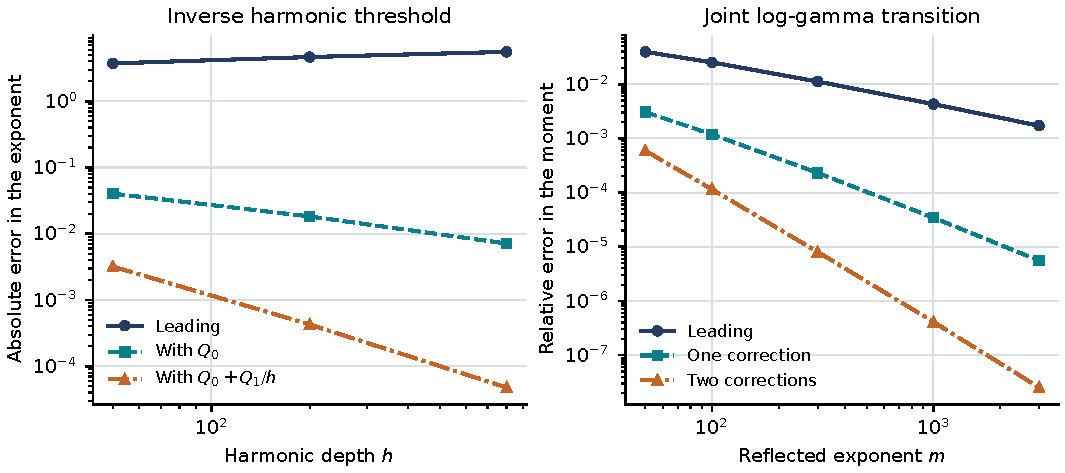
\includegraphics[width=\textwidth]{figures/correction_diagnostics.pdf}
\caption{Successive asymptotic corrections in the inverse harmonic
problem and the joint-moment transition. All plotted values are
high-precision diagnostics of the defining integrals. They are
distinct from the exact interval certificate used in the
monotonicity proof.}
\label{cont:fig:corrections}
\end{figure}

\subsection{Replay and portability}

Python 3.10 or later suffices for the supplied core scripts.
The symbolic and diagnostic programs additionally use SymPy and
mpmath; the versions used in this delivery are recorded in
\src{provenance/verification_receipt.json}. The package-level
\src{verify.py} runs the exact checks in a temporary directory,
compares the critical saved results, and records a fresh verification
receipt. Numerical diagnostics are available as an optional replay,
since they take longer and are not proof gates for the analytic
theorems. The \TeX{} source builds with a standard recent TeX Live
installation using \texttt{latexmk -pdf article.tex}.

The source receipts identify all thirty-nine inspected consolidated
source files and the six incoming archives. SHA-256 checksums cover
the delivered artifacts. These records make the scope of the audit
and the origin of the baseline unambiguous, without redistributing
the entire existing manuscript or its incoming packages.


% ===== sections/08-research-agenda.tex =====
\section{Further research questions}
\label{cont:sec:questions}

The following programme prioritizes questions for which the present
results supply a concrete starting point. Some are new refinements
of the baseline questions; others remain difficult after the
progress made here. The statements in this section are proposals,
not additional theorems.

\subsection{Harmonic sums and uniform asymptotics}

\begin{enumerate}[leftmargin=*,label=H\arabic*.]
\item \textbf{Certified relative remainders on the entire saddle
range.} The proof of Theorem~\ref{us:thm:uniform} supplies uniform
derivative and curvature control, including the explicit bound
\eqref{us:eq:curvature-bound}. Derive useful computable constants
$C_J,p_J$ such that
\[
 \left|\frac{R_{p,h}}{\mathcal S_{p,h}}
      -\sum_{j=0}^JE_jp^{-j}\right|
 \le C_Jp^{-J-1}\quad(p\ge p_J)
\]
holds for every $h\ge1,a>0$. The main task is to retain practical
constants in the Gaussian Taylor and endpoint bounds.

\item \textbf{A bridge to bounded $p$.} The new theorem is uniform
in $p/h$, but requires $p\to\infty$. Find a single approximation
which joins it to the fixed-$p$, growing-$h$ endpoint expansion.
An incomplete-gamma or gamma-density formulation may be more
natural than forcing a Gaussian approximation when its shape
parameter stays bounded.

\item \textbf{Inverse fractions approaching zero or one.}
The inverse theorem keeps $\theta$ away from both endpoints.
Determine the largest moving ranges of
$\lambda=-\log\theta$ for which the polynomial inverse remains
uniform. For example, how do the scales change if
$\lambda\to0$ or $\lambda\to\infty$ with $h$? Near the lower
endpoint $(\log2)^h/2$, the transition underlying the inverse
itself changes.

\item \textbf{Late saddle coefficients.} The all-orders expansion
is effective at every fixed order, but does not describe the growth
of $E_j$ as $j\to\infty$. Identify the complex saddles and
singularities controlling that growth, and determine whether an
optimal-truncation theorem can be uniform over the moving real
saddle. This would connect the harmonic analysis with the
manuscript's sharp reflected-moment work.
\end{enumerate}

\subsection{Two growing log-gamma exponents}

\begin{enumerate}[leftmargin=*,label=M\arabic*.]
\item \textbf{An analytic slope-ratio inequality and its sharp
constant.} Theorem~\ref{gs:thm:monotonicity} proves global
monotonicity using an exact interval certificate in the middle.
Find a proof based entirely on analytic inequalities, and determine
the optimal lower bound for $J'/J$. The symmetry suggests that
the midpoint deserves special attention, but the certificate given
here does not assert that it is the minimizer.

\item \textbf{Moving transition parameter.} Extend
Theorem~\ref{joint:thm:transition} to transition parameters which
tend to zero or infinity. Its correction polynomials exhibit
how powers of $\lambda$ compete with powers of $m^{-1}$, but
that formal observation is not a uniform bound. Determine the
first range in which the cubic and higher local perturbations
change the leading transition function.

\item \textbf{Uniform bridges between moment regimes.}
Construct an approximation valid while the dominant saddle
travels from a fixed interior point to $x\asymp m^{-1}$ and
beyond. The transition limit proved here supplies a necessary
boundary condition. A successful formula must also control the
opposite endpoint, rather than using a local series alone.

\item \textbf{A general analytic endpoint-pair theorem.}
For $f(x)=-\log x+g(x)$ and
$B(x)=b_1x+b_2x^2+\cdots$, the local argument suggests the
leading factor
\[
 \exp\bigl((g_1+b_2/b_1)\lambda\bigr).
\]
State and prove explicit global conditions under which this
generalization is valid. The exact coefficient recipe indicates
which parts are formal; the endpoint localization identifies
where additional hypotheses are needed.

\item \textbf{Optimal truncation with a growing reflected
exponent.} Determine the maximal growth of $m$ for which the
fixed-$m$ half-first-omitted-term law remains uniform. The factor
$B(-\tau)^m$ in the inverse-gamma amplitude changes the late-term
saddle. A theorem must track this effect together with the
transition polynomials, not simply substitute a variable $m$
into a fixed-amplitude estimate.
\end{enumerate}

\subsection{Integral distribution lattices}

\begin{enumerate}[leftmargin=*,label=D\arabic*.]
\item \textbf{Three or more prime divisors.} Determine
$\operatorname{coker}P_q$ integrally for squarefree $q$ with at
least three prime divisors. The two-prime core suggests an
incidence presentation involving intersections of divisor layers.
Which torsion classes require more than pairwise cycle information?

\item \textbf{Prime powers in the primitive cokernel.} Extend
the explicit classification from $p\ell$ to $p^a\ell^b$.
The full quotient already has a basis and finite resolution, so
the difficulty is the primitive inclusion. Separate the effect
of higher primary heights from multiplication-cycle torsion.

\item \textbf{An exact denominator formula for every level.}
For $q=p\ell$ the answer is a least common multiple of three
explicit factors. For general $q$, seek a formula for the exponent
of the integral primitive cokernel, rather than merely its
determinant. A product bound can exceed the needed denominator
substantially, as the level-fifteen example demonstrates.

\item \textbf{Integral reflection and jet modules.} Study
reflection quotients in characteristic two and spectral jets over
integer or finite-characteristic coefficient rings. The full
distribution module remains free, but the primitive image may
simultaneously have spectral defects and modular torsion. A
presentation that keeps both effects should be useful for
special-value computations without semisimple character projectors.
\end{enumerate}

\subsection{Gaussian polylogarithms and exact discovery}

\begin{enumerate}[leftmargin=*,label=G\arabic*.]
\item \textbf{Prove or refute the common $S_6$ conjecture.}
Use the reduced coordinate form
\eqref{s6audit:eq:reduced-candidate}. The weight-five success
indicates that transformations of iterated-integral paths can
supply information outside a restricted depth-two product module.
A successful proof must display the extra analytic relation and
an exact finite combination, not only a numerical null vector.

\item \textbf{Control relation-space growth before elimination.}
The weight-seven experiment shows how sparse rows can become
dense during elimination. Work first in shuffle indecomposables,
exploit color and reversal symmetries, and isolate the relevant
quotient before adjoining transformed paths. A modular calculation
which suggests membership should be followed by rational
reconstruction and exact verification of every relation.

\item \textbf{Obstructions with an explicit relation vocabulary.}
Extend the existing uniform depth-two obstructions to carefully
specified larger presentations. A nonzero functional on a
restricted module is useful because it identifies missing
information; it is not a theorem about all functional equations
of the evaluated periods. State the alphabet, regularization
rules, allowed depths, and parameter transformations in each
obstruction theorem.

\item \textbf{A reproducible conjecture registry.} Store each
candidate with an immutable coordinate order, a primitive integer
relation, discovery precision, frozen-coefficient reevaluation,
and its exact relations to other candidates. The two $S_6$
presentations show why coordinate equivalence should be checked
before counting independent discoveries. Keep numerical evidence,
formal proofs, and interval certificates as distinct fields.
\end{enumerate}

These questions preserve the central aim of the programme: explain
why an identity holds, identify the structure that makes it
computable, and state precisely where an argument ceases to be
uniform or a formal relation ceases to determine an arithmetic one.


% ===== references.tex =====
\begin{thebibliography}{99}
\small
\raggedright

\bibitem{cont:ProveIt}
ProveIt Contributors, \emph{Polylogarithms and their Arithmetic
Bridges: Special Values, Zeta Jets, Lattices and Experimental
Discovery}, consolidated manuscript, October 2026.
V.~Reshetnikov's ProveIt repository, commit
\texttt{cc34f73596336f2466d9754cb0f3635bd2bedade}.
\url{https://github.com/VladimirReshetnikov/ProveIt/tree/cc34f73596336f2466d9754cb0f3635bd2bedade/Analysis/Polylogarithms/docs/manuscript}.
The exact inspected file hashes accompany this article.

\bibitem{cont:RankIncoming}
ProveIt incoming research contribution,
\emph{Two Reflections and Exact Ranks for Level-Four Double Polylogarithms},
incoming research archive
\src{polylogarithms_level4_rank_2026-10-09.zip}, deposited in
\src{docs/incoming} at the commit in \cite{cont:ProveIt}.
Git blob \texttt{fcc2e2468343c31a84458fd8b3e2e32b9057a554}.
The archive includes an all-weight rank theorem and integration source.

\bibitem{cont:FormalIncoming}
ProveIt incoming research contribution,
\emph{Formal Reductions and Singular Limits in Polylogarithm Arithmetic},
incoming research archive
\src{ProveIt_Polylogarithms_Formal_Reductions_2026-10-10.zip},
\src{docs/incoming}, at the same pinned commit.
Git blob \texttt{4daeed6db6ace108abb5058e40d281846d9da381}.

\bibitem{cont:CayleyIncoming}
ProveIt incoming Cayley research contribution,
\src{proveit_cayley_s4_research.zip}, \src{docs/incoming},
at the same pinned commit.
Git blob \texttt{564459b6cf541a057d0ee8dcaa4205a824b629c8}.
The stored weight-seven relation is used here only as a conjecture.

\bibitem{cont:DLMFLaplace}
F.~W.~J. Olver, A.~B. Olde Daalhuis, D.~W. Lozier et al., eds.,
\emph{NIST Digital Library of Mathematical Functions},
\S2.3(iii), Laplace's method.
\url{https://dlmf.nist.gov/2.3#iii}. Accessed 10 October 2026.

\bibitem{joint:DLMF}
\emph{NIST Digital Library of Mathematical Functions},
\S5.7, series expansions of the gamma and psi functions.
\url{https://dlmf.nist.gov/5.7}. Accessed 10 October 2026.

\bibitem{gaussian:ACEMKM}
T.~Amdeberhan, M.~W. Coffey, O.~Espinosa, C.~Koutschan,
D.~V. Manna, and V.~H. Moll, Integrals of powers of loggamma,
\emph{Proceedings of the American Mathematical Society}
\textbf{139} (2011), no.~2, 535--545.
\href{https://doi.org/10.1090/S0002-9939-2010-10589-0}{doi:10.1090/S0002-9939-2010-10589-0}.
Author preprint:
\url{https://www.math.tulane.edu/~vhm/papers_html/lg-subm.pdf}.

\bibitem{intdist:Kubert1979}
D.~S. Kubert, The universal ordinary distribution,
\emph{Bulletin de la Soci\'et\'e Math\'ematique de France}
\textbf{107} (1979), 179--202.
\href{https://doi.org/10.24033/bsmf.1891}{doi:10.24033/bsmf.1891}.
\url{https://www.numdam.org/articles/10.24033/bsmf.1891/}.

\bibitem{intdist:Ouyang2001}
Y.~Ouyang, with an appendix by G.~W. Anderson,
Group cohomology of the universal ordinary distribution,
\emph{Journal f\"ur die reine und angewandte Mathematik}
\textbf{537} (2001), 1--32.
\url{https://arxiv.org/abs/math/9911032}.

\bibitem{intdist:Ouyang2002}
Y.~Ouyang, On the universal norm distribution,
arXiv:math/0210297v2, 2002.
In particular Proposition~4.2 and Theorem~5.1.
\url{https://arxiv.org/pdf/math/0210297}.

\bibitem{cont:Zhao}
J.~Zhao, Standard relations of multiple polylogarithm values at roots
of unity, \emph{Documenta Mathematica} \textbf{15} (2010), 1--34.
\url{https://arxiv.org/abs/0707.1459}.

\end{thebibliography}

\end{document}
